% !TEX program = xelatex
% 中文稿：Overleaf 中请将编译器设为 XeLaTeX（Menu -> Compiler -> XeLaTeX）。
\documentclass[sigconf,anonymous,review,balance=false]{acmart}

\usepackage{xeCJK}
\setCJKmainfont{FandolSong-Regular.otf}[BoldFont=FandolSong-Bold.otf,ItalicFont=FandolKai-Regular.otf]
\setCJKsansfont{FandolHei-Regular.otf}[BoldFont=FandolHei-Bold.otf]
\setCJKmonofont{FandolFang-Regular.otf}

\usepackage{graphicx}
\usepackage{booktabs}
\usepackage{microtype}
\usepackage{multirow}
\usepackage{enumitem}
\usepackage{array}
\usepackage{subcaption}
\usepackage{tabularx}
\usepackage{float}
\usepackage{placeins}
\usepackage{amsmath}
\let\Bbbk\relax
\usepackage{amssymb}
\usepackage{listings}
\usepackage{xcolor}

\settopmatter{printacmref=false,printccs=false}
\setcopyright{none}
\renewcommand\footnotetextcopyrightpermission[1]{}

\acmConference[KDD '27]{The 33rd ACM SIGKDD Conference on Knowledge Discovery and Data Mining}{August 1--5, 2027}{San Jose, CA, USA}
\acmISBN{}
\acmDOI{}
\acmYear{2027}
\copyrightyear{2027}

\newcommand{\clip}{\operatorname{clip}}
\newcommand{\sigmoid}{\operatorname{sigmoid}}
\newcommand{\ind}{\mathbf{1}}

\AtBeginDocument{%
  \providecommand\BibTeX{{Bib\TeX}}%
  \renewcommand{\abstractname}{摘要}%
  \renewcommand{\keywordsname}{关键词}%
  \renewcommand{\figurename}{图}%
  \renewcommand{\tablename}{表}%
  \renewcommand{\lstlistingname}{代码清单}%
  \renewcommand{\refname}{参考文献}}

\newcommand{\tr}[2]{#1}
\emergencystretch=1em
\begin{document}

\title[Civitas Economica：多尺度市场仿真]{Civitas Economica：融合社会心理学、金融关系与博弈论的 LLM 智能体市场社会仿真系统}

\begin{abstract}
本文提出 Civitas Economica，一个可接入 LLM 智能体的社会仿真系统，用于刻画人与人、人与群体、群体与市场制度之间经济关系的共同演化。社会心理学为注意力筛选、恐慌传染及信心依赖从众提供动机，行为金融学将持仓及多重价格参考点连接到估值，博弈论启发对共享信息、价格与交易约束下策略相互依赖的刻画。离散因果时钟、连续双向拍卖和整数账本将这些机制接入同一执行过程。数值规则、画像启发式、全量 LLM 和双速调度共用订单契约。在一个共同父世界的分支中，阻断二次传染使感染峰值由 45\% 降至 5\%，最大回撤由 0.4754\% 降至 0.1453\%。关闭从众时换手率改变，传播与从众的回撤交互项为零。停牌分支则说明，价格平稳与撮合机会需要联合观测。日内轨迹和固定观察请求分别检验市场执行与认知接口。该系统能够追踪个体状态如何经群体互动和市场制度反馈至后续决策。
\end{abstract}

\keywords{基于主体的社会仿真, 行为金融, 社会传染, LLM 智能体, 策略相互依赖, 市场微观结构}

\maketitle

\section{引言}
\label{sec:introduction}

最新成交价来自最近一次撮合。两笔成交之间，投资者仍可能接收新信息、修正交易意图并调整对同伴的依赖程度。要解释冲击后的价格变化，需要同时知道市场何时可交易、投资者如何相互影响，以及哪些信息实际进入了决策。基于主体的模型为理解个体互动如何形成市场统计特征提供了工具~\cite{cont2001empirical,lebaron2006agent,farmer2009economy,lux1999scaling}。本文关心的是，如何在同一仿真中刻画投资者之间、投资者与群体之间、群体与市场之间的经济关系，并追踪这些关系的共同演化。

\textbf{Civitas Economica} 将上述关系组织为三个尺度（图~\ref{fig:overview}）。
\begin{itemize}[leftmargin=*,itemsep=2pt]
 \item \textbf{人与人。} 持仓将金融风险与社会联系连接起来。在固定网络上，风险暴露相近的投资者获得较高的边权，注意力筛选决定哪些同伴消息进入观察。
 \item \textbf{人与群体。} 同伴接触可以传播恐慌，悲观邻居占比与个人信心调节对群体的依赖。投资者画像提供异质的角色与决策参数，群体状态在网络互动中演化。
 \item \textbf{群体与社会。} 群体的订单进入连续双向拍卖。交易制度决定哪些订单能够成交，结算后形成的价格、持仓和流动性反馈到下一步。此处社会尺度指模型内的市场集体结果。
\end{itemize}

社会心理学为注意力、情绪传染与从众提供动机~\cite{deutsch1955study,hatfield1993emotional,tajfel1979integrative}，行为金融学为持仓、价格参考点与估值之间的关系提供依据~\cite{kahneman1979prospect,tversky1992advances}。博弈论启发了对策略相互依赖的刻画：一个投资者的行动会改变他人面对的信息、价格与约束~\cite{cooper1988coordinating,keynes1936general,morris2002social}。系统将这些通道写成可执行的行为更新和市场规则。在同一观察与订单契约下，数值规则、画像启发式、全量 LLM 与双速混合策略均可接入这个闭环。

\subsection{研究问题}
\label{sec:rq_zh}

\begin{itemize}[leftmargin=*,itemsep=3pt]
 \item \textbf{市场活动（RQ1）。} 在相同的撮合规则与稀疏激活下，不同行为规则生成怎样的交易活动与盘口覆盖？
 \item \textbf{跨尺度反馈（RQ2）。} 从共同市场状态出发，恐慌传播、信心依赖从众、估值与监管规则如何改变社会状态、价格与交易机会？
 \item \textbf{决策接口与调度（RQ3）。} 在固定观察中，不同后端如何响应价格、锁仓与现金变化？周期式 LLM 调度如何影响请求机会与公告文字曝光？
\end{itemize}

\subsection{本文主要贡献}
\label{sec:contributions_zh}

\begin{itemize}[leftmargin=*,itemsep=2pt]
 \item \textbf{显式的三层经济关系模型。} 风险暴露塑造同伴关系，群体状态进入估值与订单意图，市场出清再改变主体在下一步面对的价格与持仓。
 \item \textbf{异质主体共用的执行环境。} 因果时钟规定信息可见性，整数账本按同一规则预留资源并执行结算。双速策略缓存方向与资源比例，并用当步价格与余额重新生成订单。
 \item \textbf{可追踪的跨尺度比较。} 共同检查点分支使行为机制与制度规则可分别干预，并记录从社会状态到交易的路径。本文结合日内流动性记录、分画像的动作差异和运行计时检验这一设计。
\end{itemize}

\section{相关工作}
\label{sec:related}

\subsection{行为金融与社会关系}

前景理论刻画参考依赖、损失厌恶与边际敏感性递减~\cite{kahneman1979prospect,tversky1992advances}。心理账户与内生参考点解释同一价格如何对应不同的评价基准~\cite{thaler1985mental,koszegi2006model}；处置效应则为区分持仓成本与当前价格提供动机~\cite{shefrin1985disposition,odean1998reluctant}。Civitas 将这些金融状态与人与人的关系相连：风险暴露相似度调整既有社会联系的权重，持仓成本、近期高点、同伴共识与政策信号共同进入参考依赖估值。

社会心理学研究群体归属、情绪传染以及信息性和规范性影响~\cite{tajfel1979integrative,hatfield1993emotional,deutsch1955study}。小世界连通结构与选择性接触启发了联系网络和信息获取的建模~\cite{watts1998collective,sunstein2001republic}。在人与群体尺度上，Civitas 通过注意力受限的消息筛选与同步恐慌状态转移更新局部社会状态，由信心调节同伴权重。投资者画像规定异质角色，并与网络位置独立设置；模型中的群体反馈通过邻域互动形成。

\subsection{协调行为与市场制度}

战略互补性、对他人估值的预期和公共信息博弈刻画协调激励~\cite{cooper1988coordinating,keynes1936general,morris2002social}。信息级联模型解释先前行动如何影响后续决策~\cite{bikhchandani1992theory,banerjee1992simple}，噪声交易者风险与套利限制解释价格偏离为何可能持续~\cite{delong1990noise,shleifer1997limits}。这些理论为 Civitas 中依赖同伴的更新规则提供动机，仿真沿给定的行为动态逐步推进。群体与社会尺度对应模型内的市场制度：群体订单形成价格与交易机会，并反馈到个体决策。

交易机制规定上述聚合过程。零智能实验分离出预算约束与双向拍卖规则的作用~\cite{gode1993allocative}；图表派与基本面派交互模型生成厚尾收益与波动率聚集~\cite{lux1999scaling,lux2000volatility,raberto2001agent}。市场微观结构理论将价格形成与信息不对称联系起来~\cite{kyle1985continuous,glosten1985bid}。ABIDES 提供带可配置通信延迟和可编程主体的离散事件限价订单簿~\cite{abides2020}。Civitas 先在离散决策时点统一可见信息，再将订单依次送入连续双向拍卖撮合。

\subsection{市场仿真中的大语言模型}

生成式主体通过语言理解观察并扮演角色~\cite{park2023generative}。金融应用包括 FinMem 的分层记忆、FinAgent 的多模态信号与工具，以及 StockAgent 和 TradingAgents 的角色化交易~\cite{yu2023finmem,zhang2024finagent,li2024stockagent,xiao2024tradingagents}。EconAgent 刻画家庭劳动与消费~\cite{li2024econagent}。TwinMarket 将信念--愿望--意图投资者及社会信息接入集合竞价~\cite{yang2025twinmarket}。MarketSim 在连续双向拍卖中分离战略层 LLM 决策与高频执行~\cite{marketsim2026}。StockSim 提供包含两种执行设置、延迟与滑点的订单级 LLM 评估环境~\cite{papadakis2025stocksim}。

表~\ref{tab:related_comparison} 分别对照交易机制、社会与行为机制、决策组织以及评估重点。Civitas 将可独立调节的社会与估值规则、整数记账和共同状态分支结合起来，在共用决策契约下追踪人际接触与群体反馈如何进入订单意图及最终执行。

\begin{table*}[t]
  \centering\small
  \setlength{\tabcolsep}{4pt}
  \caption{\tr{金融市场仿真平台的设计与评估重点。各项概括所引文献报告的功能与研究重点。}{Design and evaluation focus of financial market simulators. Entries summarize features and study emphases reported in the cited work.}}
  \label{tab:related_comparison}
  \begin{tabularx}{\textwidth}{@{}>{\raggedright\arraybackslash}p{1.95cm} >{\raggedright\arraybackslash}p{2.65cm} >{\raggedright\arraybackslash}p{3.5cm} >{\raggedright\arraybackslash}p{3.3cm} >{\raggedright\arraybackslash}X@{}}
    \toprule
    \tr{平台}{Platform} & \tr{交易机制}{Exchange} & \tr{社会与行为机制}{Social / behavioral layer} & \tr{决策组织}{Decision organization} & \tr{评估与审计重点}{Evaluation and audit focus} \\
    \midrule
    \textbf{ABIDES}\newline\cite{abides2020} & \tr{离散事件限价订单簿；通信延迟}{Discrete-event limit order book; communication latency} & \tr{背景交易者与策略交易者}{Background and strategic traders} & \tr{可编程主体策略}{Programmable agent policies} & \tr{订单与消息记录；交易实验}{Order and message traces; trading experiments} \\
    \addlinespace
    \textbf{TwinMarket}\newline\cite{yang2025twinmarket} & \tr{日级集合竞价}{Daily call auction} & \tr{交易相似度社会信息流；谣言传播}{Trading-similarity social feed; rumor diffusion} & \tr{基于信念--愿望--意图的 LLM 投资者}{Belief--desire--intention LLM investors} & \tr{风格化事实与社会响应场景}{Stylized facts and social-response scenarios} \\
    \addlinespace
    \textbf{MarketSim}\newline\cite{marketsim2026} & \tr{纳秒精度连续双向拍卖}{Nanosecond-resolution continuous double auction} & \tr{异质投资者；新闻与政策信息}{Heterogeneous investors; news and policy information} & \tr{战略层 LLM 决策与快速执行层}{Strategic LLM decisions with a faster execution layer} & \tr{风格化事实与高频价格跟踪}{Stylized facts and high-frequency price tracking} \\
    \addlinespace
    \textbf{StockSim}\newline\cite{papadakis2025stocksim} & \tr{订单级执行；延迟与滑点}{Order-level execution; latency and slippage} & \tr{异质交易角色与多主体协调}{Heterogeneous trading roles and multi-agent coordination} & \tr{两种执行设置下的 LLM 交易决策}{LLM trading decisions in two execution settings} & \tr{序列交易决策评估}{Sequential trading decision evaluation} \\
    \addlinespace
    \textbf{Civitas Economica} & \tr{同步决策；连续双向拍卖；整数结算}{Synchronous decisions; continuous double auction; integer settlement} & \tr{暴露加权联系；参考点估值；恐慌与从众}{Exposure-weighted ties; reference valuation; panic and herding} & \tr{共用契约下的规则、启发式、LLM 与双速策略}{Shared contract for rules, heuristics, LLM, and dual-speed policies} & \tr{共同状态分支；账本与接口检查}{Shared-state branches; ledger and interface checks} \\
    \bottomrule
  \end{tabularx}
\end{table*}


\section{方法：Civitas Economica 框架}
\label{sec:method}

Civitas Economica 在同一时钟下连接人与人的联系、人与群体的相互影响，以及群体与社会尺度的市场结果。图~\ref{fig:overview} 从可见观察出发，经估值与订单推进到结算，再将价格与持仓反馈至下一步。设主体总数为 $N$，主体索引为 $i,j\in\{1,\dots,N\}$，仿真步为 $t\in\{1,\dots,T\}$。截断算子为 $\clip(x,l,u)=\max(l,\min(u,x))$，标准 Logistic 函数为 $\sigma(x)=(1+e^{-x})^{-1}$。市场交易单一风险资产与无风险现金。每张订单均以可用现金或可卖持仓为上限，市场禁止无抵押借贷和裸卖空。

\begin{figure*}[t]
  \centering
  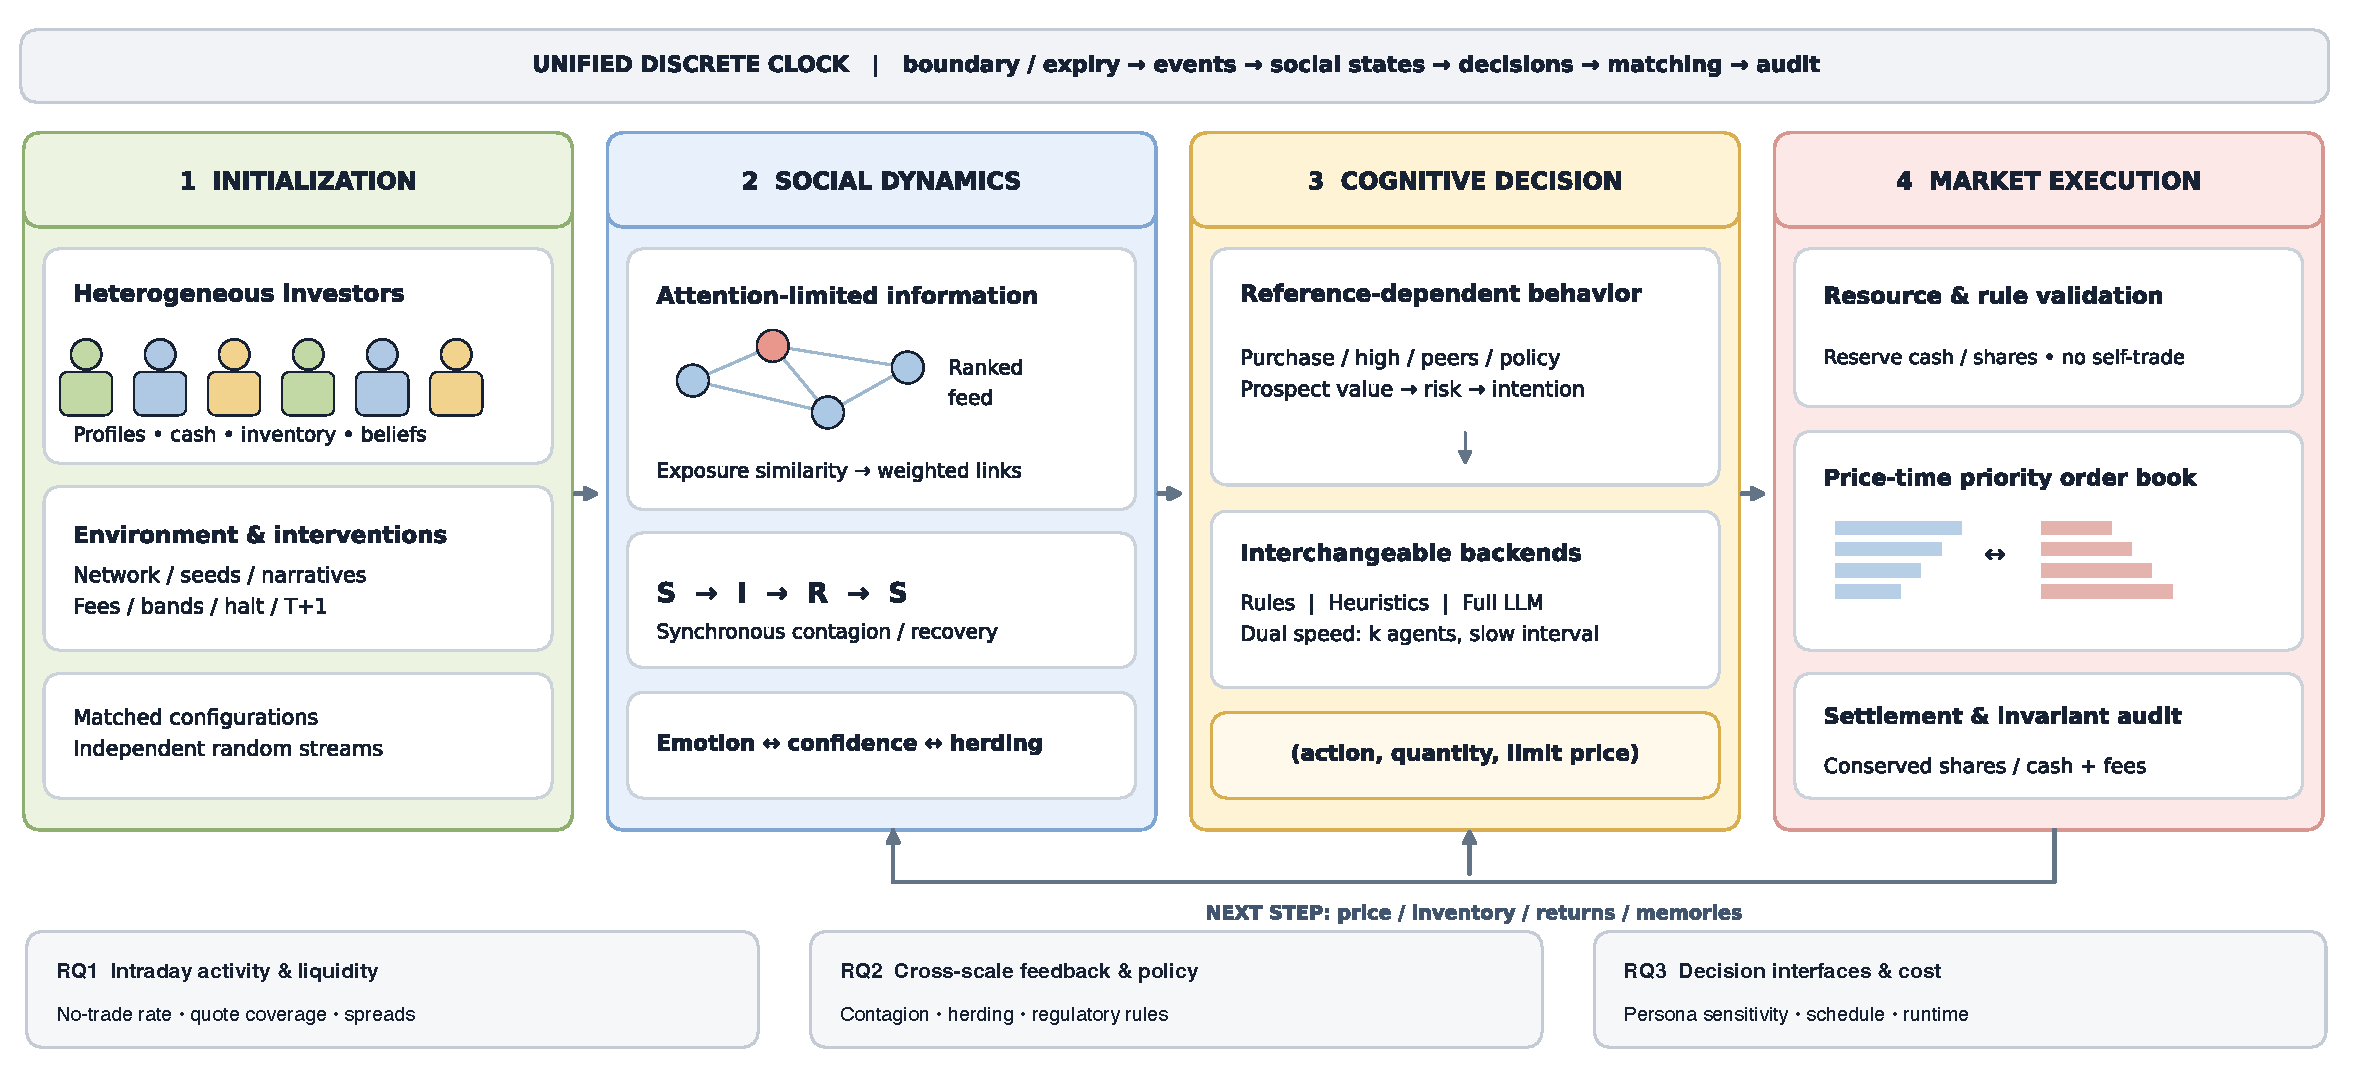
\includegraphics[width=\textwidth]{figures/fig1_methodology_overview.pdf}
  \caption{Civitas Economica 架构。持仓风险暴露调节同伴边权，群体状态参与形成委托，结算产生新的价格和持仓。阶段 \ref{phase:boundary_zh}--\ref{phase:events_zh} 完成市场准备，阶段 \ref{phase:social_zh}--\ref{phase:behavior_zh} 按式~\eqref{eq:exposure_zh}--\eqref{eq:confidence_update_zh} 更新信息与行为状态。阶段 \ref{phase:decision_zh} 通过式~\eqref{eq:aggregate_v_zh}--\eqref{eq:order_quantity_zh} 或认知接口生成委托，接口支持式~\eqref{eq:cache_signature_zh} 的缓存。阶段 \ref{phase:execution_zh}--\ref{phase:commit_zh} 按种子确定的顺序接收委托，并按式~\eqref{eq:settle_b_zh}--\eqref{eq:invariants_zh} 结算与提交。}
  \Description{八阶段时钟连接同伴暴露、群体状态、订单与市场结算，并将结果反馈至下一步，构成三个经济关系尺度。}
  \label{fig:overview}
\end{figure*}

\subsection{统一离散时钟与严格因果调度}
\label{sec:method:clock_zh}

每个仿真步 $t$ 按以下八个阶段推进，以确定各字段何时可见。
\begin{enumerate}[leftmargin=*, label=(\arabic*), ref=\arabic*]
  \item\label{phase:boundary_zh} \textbf{交易日边界与涨跌幅基准重置。} 首日以 $P_0$ 初始化。随后每个交易日首步（$t>1$ 且 $(t-1)\bmod T_{\mathrm{day}}=0$），锚定基准价 $P^{\mathrm{base}}_t = P_{t-1}$，计算日内价格区间 $[P_t^{\mathrm{lower}}, P_t^{\mathrm{upper}}] = [P^{\mathrm{base}}_t(1-L), P^{\mathrm{base}}_t(1+L)]$，并解除到期的持仓锁定。
  \item\label{phase:expiry_zh} \textbf{订单到期与资源释放。} 撤销到期挂单，将剩余预留现金与股份归还可用账本。
  \item\label{phase:events_zh} \textbf{外生事件与公共叙事。} 向公共信息池发布预定的宏观公告、企业财报或监管冲击。
  \item\label{phase:social_zh} \textbf{社会交互与信息筛选。} 按风险暴露相似度更新边权，按注意力容量筛选消息，依据事件处理后的邻居状态同步更新 SIRS 状态。
  \item\label{phase:behavior_zh} \textbf{情绪与信心更新。} 先由上一步信心与悲观邻居占比计算从众权重，再用转移后的感染态、上一步同伴情绪与收益更新 $s_{i,t}$，并按从众触发状态更新信心 $q_{i,t}$。
  \item\label{phase:decision_zh} \textbf{认知决策。} 所有主体均更新参考点。活跃掩码 $A^{\mathrm{act}}_{i,t}\sim\mathrm{Bernoulli}(p_{\mathrm{act}})$ 在主体与步之间抽样，并在匹配比较中共享。活跃主体调用指定后端，输出 \texttt{(action, quantity, price)}，非活跃主体提交 \texttt{HOLD}。
  \item\label{phase:execution_zh} \textbf{订单校验、撮合与结算。} 按共享种子生成的到达顺序处理订单，核验现金或可卖股份。可接受订单在簿内按价格--时间优先撮合，再结算成交和费用。
  \item\label{phase:commit_zh} \textbf{账本审计与状态记录。} 检查现金与股份守恒，记录交易、账本和主体状态。
\end{enumerate}

认知后端接收上一提交步的价格与盘口、当步自身可用资源和心理状态，以及当步已发布事件。自己的执行回执从第 $t+1$ 步可见。单步有效期下，未成交挂单在下一步的阶段（\ref{phase:expiry_zh}）到期，历史盘口作为当步决策的观察值。

\subsection{三层演化尺度与多原型画像}
\label{sec:method:population_zh}

\paragraph{人与人} 点对点联系的权重随风险暴露相似度更新。第 $t-1$ 步结算后，主体 $i$ 的现金与股份分别为 $C_{i,t-1}$ 和 $Q_{i,t-1}$。风险资产暴露定义如下。
\begin{equation}
x^{\mathrm{exp}}_{i,t-1}=\frac{Q_{i,t-1}P_{t-1}}{C_{i,t-1}+Q_{i,t-1}P_{t-1}+\epsilon}.
  \label{eq:exposure_zh}
\end{equation}
主体 $i$ 与邻居 $j$ 的边权向由资产配置相似度决定的目标值平滑更新。
\begin{equation}
\begin{split}w_{ij,t}=\clip\bigl(&(1-\omega)w_{ij,t-1}\\&+\omega(2-|x_i^{\rm exp}-x_j^{\rm exp}|),w_{\min},w_{\max}\bigr).\end{split}
  \label{eq:edge_weight_zh}
\end{equation}
式中 $x_i^{\rm exp}$ 与 $x_j^{\rm exp}$ 均取 $t-1$ 步，$\omega=0.1$，$(w_{\min},w_{\max})=(1,2)$。$\epsilon>0$ 使零财富时的暴露有定义，现金与价格采用同一计价单位。风险敞口越接近，边权的目标值越高。这些边权用于邻域汇总，式~\eqref{eq:message_score_zh} 则在有限注意力下筛选具体消息来源。

\paragraph{人与群体} 筛选后的消息与加权邻域状态经式~\eqref{eq:infection_prob_zh}--\eqref{eq:confidence_update_zh} 更新感染、情绪与信心。九类画像的抽样概率为散户 70\%、公募基金 8\%、养老金 5\%、保险机构 4\%、自营交易台 4\%、做市商 4\%、平准资金 1\%、谣言敏感者 2\% 及套利者 2\%。画像提供角色标签与第~\ref{sec:method:cognition_zh} 节的画像决策参数，并与 Watts--Strogatz 小世界网络独立抽样~\cite{watts1998collective}。这一设置使画像与网络位置可分别调整。各画像的基准损失厌恶系数为 $2.25$。

\paragraph{群体与社会} 这一尺度表示模型市场中的集体结果。各画像的订单在共同交易规则下进入限价订单簿，形成成交价、成交量、报价价差与深度。式~\eqref{eq:settle_b_zh}--\eqref{eq:invariants_zh} 的结算改变持仓，价格与收益进入下一步的暴露、参考点和情绪更新，从而闭合市场结果到个体决策的反馈。

\subsection{社会层：注意力受限传播与信心依赖从众}
\label{sec:method:social_zh}

\paragraph{注意力受限的信息流排名} 设 $\mathcal N_i$ 为主体 $i$ 的邻域。在阶段（\ref{phase:social_zh}），主体对事件处理后处于感染态的邻居消息计算排序分数。
\begin{equation}
\begin{split}h_{ij,t}={}&\theta_1(1-|s_i-s_j|/2)+\theta_2\ind\{u_i=u_j\}\\&+\theta_3(1-|a_i-a_j|)+\theta_4 Inf_j+\theta_5 E_{ij,t-1}.\end{split}
  \label{eq:message_score_zh}
\end{equation}
五项依次为情绪相似度、主题一致性、风险偏好相似度、来源影响力和历史曝光。情绪与风险偏好取上一提交步，非负权重之和为 1。按分数选取至多 $A_i$ 个来源，形成消息集合 $\mathcal F_{i,t}$，同分按固定来源编号排序。

\paragraph{同步 SIRS 恐慌传染动力学} 模型用易感（$S$）、感染（$I$）和恢复（$R$）表示恐慌状态。感染压力由全邻域的加权感染比例与经注意力筛选的消息共同决定。
\begin{equation}
\begin{split}\rho_{i,t}&=\frac{\sum_j w_{ij,t}\ind\{\widetilde X_{j,t}=I\}}{\sum_jw_{ij,t}},\\p^{\rm inf}_{i,t}&=\clip\bigl(\overline{h_{ij,t}\mathrm{sim}_{ij,t}}_{\mathcal F_{i,t}}(\kappa_0+\kappa_1\rho_{i,t})\\&\hspace{5em}+\kappa_2\rho_{i,t},0,1\bigr).\end{split}
  \label{eq:infection_prob_zh}
\end{equation}
其中 $\widetilde X$ 为事件处理后、同步转移前的状态，$\mathrm{sim}_{ij,t}=1-|s_i-s_j|/2$，情绪取上一提交步。$\rho_{i,t}$ 在 $\mathcal N_i$ 内求和，横线表示对 $\mathcal F_{i,t}$ 中各消息的 $h_{ij,t}\mathrm{sim}_{ij,t}$ 取算术平均。空消息集的均值与空邻域的感染比例均置零。易感者以 $\clip(\beta p^{\rm inf}_{i,t}c_i,0,1)$ 的概率感染，$c_i$ 为从众倾向。感染者的恢复概率由当前感染时长和曝光集中度决定。
\begin{equation}
p^{\rm rec}_{i,t}=\clip\bigl(\gamma(1+\eta_d\widetilde D_{i,t})(1-\eta_e e_{i,t}),0,1\bigr).
  \label{eq:recovery_prob_zh}
\end{equation}
曝光记忆按 $E_{ij,t}=(1-\zeta_E)E_{ij,t-1}+\zeta_E\ind\{j\in\mathcal F_{i,t}\}$ 更新，集中度为 $e_{i,t}=\sum_j(E_{ij,t}/\sum_k E_{ik,t})^2$，总曝光为零时取 $e_{i,t}=0$。$\widetilde D$ 为转移前感染时长。恢复者以 $\clip(\delta(1+\eta_\psi p^{\rm inf}_{i,t}),0,1)$ 的概率重返易感态。各主体从转移前状态同步抽样，每步执行至多一次状态转移。

\paragraph{信心依赖的从众反馈} 连续情绪 $s_{i,t}\in[-1,1]$ 由自我惯性、感染状态、同伴情绪和市场收益共同更新。
\begin{equation}
\begin{split}s_{i,t}=\clip\bigl(&(w_i^D-\Delta_{i,t})s_{i,t-1}-w_i^g\ind\{X_{i,t}=I\}\\&+(w_i^N+\Delta_{i,t})\bar s^N_{i,t-1}\\&+w_i^M\clip(r_{t-1}/r_*,-1,1)+\epsilon_s,-1,1\bigr).\end{split}
  \label{eq:sentiment_update_zh}
\end{equation}
同伴情绪为邻居上一步情绪的边权加权均值，孤立主体取自身上一步情绪，$\epsilon_s\sim\mathcal N(0,\sigma_s^2)$。从众反馈在自我惯性和同伴共识之间重新分配权重，保持两者的总权重~\cite{deutsch1955study}。
\begin{equation}
\Delta_{i,t}=H_{i,t}\eta_H(1-q_{i,t-1})w_i^D,\qquad H_{i,t}=\ind\{b^N_{i,t}>0.5\}.
  \label{eq:herding_shift_zh}
\end{equation}
$b^N_{i,t}$ 为情绪低于 $-s_*$ 的邻居所占边权比例。从众触发时信心衰减，其余时间向 $q_0$ 恢复。消融令 $\eta_H=\eta_q=0$，并保留信心恢复项。
\begin{equation}
\begin{split}q_{i,t}=\clip\bigl(&q_{i,t-1}-H_{i,t}\eta_q(1-q_{i,t-1})\\&+(1-H_{i,t})\eta_{\rm rec}(q_0-q_{i,t-1}),0,1\bigr).\end{split}
  \label{eq:confidence_update_zh}
\end{equation}

\subsection{行为核心：多参考点前景理论与订单映射}
\label{sec:method:behavior_zh}

\paragraph{四重自适应参考点} 社会状态更新后，主体在阶段（\ref{phase:decision_zh}）更新持仓成本（$R^p$）、滚动局部高点（$R^h$）、同伴共识（$R^n$）和政策信号（$R^e$）四类心理锚点。
\begin{align}
 R^p_{i,t}&=(1-\kappa_p)R^p_{i,t-1}+\kappa_p T^p_{i,t},\label{eq:ref_p_zh}\\
 R^h_{i,t}&=(1-\kappa_h)R^h_{i,t-1}+\kappa_h \max_{v=\max(0,t-H_h)}^{t-1}P_v,\label{eq:ref_h_zh}\\
 R^n_{i,t}&=(1-\kappa_n)R^n_{i,t-1}+\kappa_nP_{t-1}(1+\xi_n\bar s^N_{i,t-1}),\label{eq:ref_n_zh}\\
 R^e_{i,t}&=(1-\kappa_e)R^e_{i,t-1}+\kappa_eP_{t-1}(1+\xi_e u_t^{\rm policy}).\label{eq:ref_e_zh}
\end{align}
持仓非零时，成本目标为 $T^p=K$，其中 $K$ 为不含费用的持仓成本价。空仓时取 $T^p=P_{t-1}$。政策状态持续至新事件覆盖，事件文本在发布当步可见。

\paragraph{前景价值与动态损失压力} 参考偏差通过非对称幂函数映射为前景价值~\cite{tversky1992advances}。
\begin{equation}
v_i(z)=\begin{cases}z^\alpha&z\ge0,\\-\lambda_i(-z)^\alpha&z<0.\end{cases}
  \label{eq:prospect_v_zh}
\end{equation}
基准设定中 $\lambda_i>1$ 刻画损失厌恶，$\alpha\in(0,1)$ 刻画边际敏感性递减。成本与高点采用回顾性偏差，同伴与政策采用前瞻性偏差。先聚合四类偏差，再计算前景价值与估值方向。
\begin{equation}
\begin{split}x^\bullet_{i,t}&=\begin{cases}(P_{t-1}-R^\bullet_{i,t})/R^\bullet_{i,t}&\bullet=p,h,\\(R^\bullet_{i,t}-P_{t-1})/P_{t-1}&\bullet=n,e,\end{cases}\\z_{i,t}&=\sum_\bullet\omega_\bullet x^\bullet_{i,t},\quad V_{i,t}=v_i(z_{i,t}),\quad d_{i,t}=\tanh(\kappa_vV_{i,t}).\end{split}
  \label{eq:aggregate_v_zh}
\end{equation}
回顾性浮亏比例 $b_{i,t}=(\omega_p\mathbf{1}\{P_{t-1}<R^p_{i,t}\}+\omega_h\mathbf{1}\{P_{t-1}<R^h_{i,t}\})/(\omega_p+\omega_h)$ 衡量价格低于成本或高点的参考权重份额，进入有界的损失压力函数。
\begin{equation}
  \ell_{i,t} = \clip\left( \lambda_i (1 + \chi b_{i,t}), \ell_{\min}, \ell_{\max} \right).
  \label{eq:loss_pressure_zh}
\end{equation}
当前风险偏好 $a_{i,t}\in[0,1]$ 结合信心、上一步风险偏好、情绪、估值方向与损失压力。
\begin{equation}
\begin{split}a_{i,t}=\clip\bigl(&\omega_a^q q_{i,t}+\omega_a^a a_{i,t-1}+\omega_a^s s_{i,t}\\&+\omega_a^d d_{i,t}-\omega_a^\ell\max(0,(\ell_{i,t}-1)/\nu),0,1\bigr).\end{split}
  \label{eq:risk_tolerance_zh}
\end{equation}

\paragraph{交易意图与限价单生成} 估值方向、情绪与风险偏好共同决定交易意图 $\tau_{i,t}\in[-1,1]$。
\begin{equation}
\tau_{i,t}=\clip\bigl(\omega_\tau^d d_{i,t}+\omega_\tau^s s_{i,t}+\omega_\tau^a(a_{i,t}-0.5),-1,1\bigr).
  \label{eq:intent_score_zh}
\end{equation}
在阈值 $\delta_a\ge0$ 下，按以下概率抽样买入、卖出或观望。
\begin{equation}
\begin{split}p_i^b&=\sigma(\kappa_a(\tau_{i,t}-\delta_a)),\\p_i^s&=\sigma(-\kappa_a(\tau_{i,t}+\delta_a)),\qquad p_i^h=1-p_i^b-p_i^s.\end{split}
  \label{eq:action_selection_zh}
\end{equation}
独立随机变量 $U_i\sim U(0,1)$ 决定买入比例 $f_i^b=U_i[f_{\min}+(f_{\max}-f_{\min})a_i]$ 和卖出比例 $f_i^s=U_i[f_{\min}+(f_{\max}-f_{\min})\max(-\tau_i,0)]$。均值校正的对数正态报价扰动独立于动作方向，并在规则基线间共享。
\begin{equation}
\begin{split}\widetilde p_i&=P_{t-1}\exp(\epsilon_p-\sigma_p^2/2),\\p_i^{\rm lim}&=\Delta_p\max\{1,\operatorname{round}_{\rm even}(\widetilde p_i/\Delta_p)\}.\end{split}
  \label{eq:limit_price_zh}
\end{equation}
其中 $\epsilon_p\sim\mathcal N(0,\sigma_p^2)$，刻度取整平局时取偶数，超出当日价带的委托直接拒收。数量按当前可用资源向下取整。
\begin{equation}
  n_i = \begin{cases}
    \bigl\lfloor f^b_{i,t} C_{i,t}^{\mathrm{free}} / \bigl(p_i^{\mathrm{lim}}(1+c)\bigr) \bigr\rfloor & \mathrm{BUY}, \\
    \bigl\lfloor f^s_{i,t} Q_{i,t}^{\mathrm{free}} \bigr\rfloor & \mathrm{SELL}.
  \end{cases}
  \label{eq:order_quantity_zh}
\end{equation}
其中 $c$ 为单侧佣金率，$C^{\rm free}$ 采用与报价一致的元单位。零数量转为 \texttt{HOLD}。

\subsection{市场微观结构与严格守恒审计}
\label{sec:method:microstructure_zh}

\paragraph{资金预留与双向撮合} 买单按限价名义额与买方佣金预留现金，卖单预留可卖股数。账本以每元 $10^6$ 个微元记账，即 $C_{i,t}^{\rm minor}=10^6 C_{i,t}$；成交名义额与费用采用同一微元单位。对整数成交名义额 $V$，每侧佣金为 $f_c=\lfloor cV\rfloor$，卖方印花税为 $f_\tau=\lfloor\tau^{\rm tax}V\rfloor$。

买单按价格降序、卖单按价格升序排列，同价按到达顺序优先，并以已有挂单价格成交。成交 $q^*$ 股时，买方 $b$、卖方 $s$ 与费用账户 $F^{\rm minor}$ 更新为
\begin{align}
  C_b^{\rm minor} &\gets C_b^{\rm minor} - V-f_c, \quad Q_b \gets Q_b + q^*, \label{eq:settle_b_zh} \\
  C_s^{\rm minor} &\gets C_s^{\rm minor} + V-f_c-f_\tau, \quad Q_s \gets Q_s - q^*, \label{eq:settle_s_zh} \\
  F^{\rm minor} &\gets F^{\rm minor} +2f_c+f_\tau. \label{eq:settle_fees_zh}
\end{align}
成交后释放对应成交数量的多余预留，剩余未成交数量的资源继续预留，直至成交、撤销或到期。

\paragraph{账本守恒} 预留资源仍属于账户余额。内核在每个提交步检查主体与费用账户的现金总和，以及主体的股份总量。
\begin{equation}
\begin{aligned}
 \sum_i C_{i,t}^{\rm minor}+F_t^{\rm minor}&=\sum_i C_{i,0}^{\rm minor}+F_0^{\rm minor},\\
 \sum_{i=1}^N Q_{i,t}&=\sum_{i=1}^N Q_{i,0}.
\end{aligned}
  \label{eq:invariants_zh}
\end{equation}
任何非零残差均触发审计错误。

\subsection{认知架构与双速混合调度}
\label{sec:method:cognition_zh}

各后端共享信息字段资格，并输出标准化的 \texttt{(action, quantity, price)}。订单校验和撮合由同一执行内核处理。
\begin{enumerate}[leftmargin=*, label=(\arabic*)]
  \item \textbf{数值规则（System 1）。} 评估公式~(\ref{eq:exposure_zh})--(\ref{eq:order_quantity_zh})，作为规则基线。
  \item \textbf{画像启发式。} 根据估值、趋势与情绪调整各画像的目标持仓比例，并用调整阈值与资源上限决定委托。
  \item \textbf{全量 LLM（System 2）。} 将主体画像、账户状态、市场事实与符合可见条件的记录序列化。接口校验响应身份与动作类型，并检查 \texttt{evidence\_ids} 无重复且属于可见 ID 集合。交易所在执行阶段核验价带与可用资源。
  \item \textbf{双速混合调度。} 全体主体执行轻量的 System 1 状态更新。系统固定选择按画像分层抽样的 $k$ 个主体，在其活跃且 $t\bmod T_{\mathrm{slow}}=0$ 时请求 System 2 响应。
\end{enumerate}

市场运行器执行规则决策、受控合成响应和归档响应。真实模型请求通过独立的固定观察工具测试同一决策契约。

\paragraph{资源自适应策略缓存} System 2 请求步缓存标准化方向与资源承诺比例，使后续订单适应当步价格和余额。
\begin{equation}
\begin{aligned}
 \widehat d_i &=
 \begin{cases}
   +1 & \mathrm{BUY}, \\
   -1 & \mathrm{SELL}, \\
   0 & \mathrm{HOLD},
 \end{cases} \\
 \widehat f_i &=
 \begin{cases}
   \min\!\bigl(1,n_i/M_i^{\mathrm{action}}\bigr) & M_i^{\mathrm{action}}>0, \\
   0 & \mbox{其他情况。}
 \end{cases}
\end{aligned}
  \label{eq:cache_signature_zh}
\end{equation}
其中 $M_i^{\mathrm{action}}$ 为按请求限价和连续佣金预算界计算的保守容量，\texttt{HOLD} 的资源承诺为零。复用时，活跃主体保持 $\widehat d_i$ 与 $\widehat f_i$，以共同报价扰动围绕 $P_{t'-1}$ 生成新限价，再将承诺比例乘以当前容量并向下取整。缓存可在年龄 $1$ 至 $A_{\max}$ 步间复用，含两端。缺失或过期时使用规则后端。已知响应异常清除缓存并提交 \texttt{HOLD}；复用后的最终数量为零时也提交 \texttt{HOLD}。

\paragraph{模型请求的调度预算} 全量 LLM 调度在 $T$ 步内提供的期望请求机会为 $p_{\mathrm{act}}NT$，双速调度为 $p_{\mathrm{act}}k\lfloor T/T_{\mathrm{slow}}\rfloor$。两者之比近似为
\begin{equation}
  \text{请求机会比} \approx \frac{k}{N \cdot T_{\mathrm{slow}}}.
  \label{eq:cost_ratio_zh}
\end{equation}
当 $N=100$、$k=10$、$T_{\rm slow}=10$ 且期限为周期整数倍时，期望请求机会减少 99\%。首个请求窗口在 $T_{\rm slow}$，固定周期调度只在预定窗口请求。实测成本按实际用量和耗时统计。
\paragraph{分析工具} OpenAI Codex 辅助实现与公式比对、归档核对和稿件整理。论文的实测分析与图表依据可追溯的归档记录。

\section{实验评估}
\label{sec:experiments_zh}

\subsection{基准配置与执行核验}
\label{sec:setup_zh}

表~\ref{tab:measured_design}所列基准从观察到的价格向上游追溯。日内轨迹（RQ1）在匹配随机流下度量成交频率和双边盘口覆盖率，区分何时有新成交、何时有双边报价可计算价差。共同父世界分支（RQ2）追踪同一感染事件后的社会状态，并检验行为机制与监管制度如何改变委托和成交。固定观察与调度核对（RQ3）进一步考察不同后端如何由观察生成意图，以及哪些计划请求有机会收到公开公告。规则世界的运行剖面度量保存和核验状态历史所需的开销。

\begin{table*}[t]
  \centering\small
  \caption{\tr{实测基准及离线调度核对的配置。长周期参考配置见附录~\ref{app:benchmark_details_zh}。}{Settings for the Measured Benchmarks and Offline Schedule Audit. Appendix~\ref{app:benchmark_details} gives the prospective long-horizon configuration.}}
  \label{tab:measured_design}
  \begin{tabularx}{\textwidth}{@{}p{0.24\textwidth} p{0.28\textwidth} X@{}}
    \toprule
    \tr{评估任务}{Evaluation} & \tr{执行配置}{Settings} & \tr{比较单位}{Unit of comparison} \\
    \midrule
    \tr{日内交易活动（RQ1）}{Intraday activity (RQ1)} &
    $N=100$, $T=T_{\rm day}=100$, $p_{\rm act}=0.05$ &
    \tr{三个匹配种子，各比较三种规则策略。}{Three matched seeds, each shared by three rule policies.} \\
    \tr{共同父世界分支（RQ2）}{Shared-parent branches (RQ2)} &
    $N=20$, $T_{\rm day}=4$, $p_{\rm act}=1$, \tr{27 步事件窗}{27 event steps} &
    \tr{一个父世界，十一条分支。}{Eleven branches from one parent world.} \\
    \tr{固定观察（RQ3）}{Fixed observations (RQ3)} &
    \tr{九类画像 $\times$ 三类对比 $\times$ 两个状态}{Nine archetypes $\times$ three contrasts $\times$ two states} &
    \tr{54 次真实 LLM 请求，构成 27 对比较。}{54 live LLM requests, organized into 27 pairs.} \\
    \tr{离线调度核对（RQ3）}{Offline scheduling (RQ3)} &
    $N=100$, $p_{\rm act}=0.05$, $k=10$, $T_{\rm slow}=10$ &
    \tr{20 个固定种子在公告发布步的计划资格。}{Scheduled eligibility at announcement release across 20 fixed seeds.} \\
    \tr{规则运行剖面（RQ3）}{Rule profiles (RQ3)} &
    \tr{同一平台 $N=100$、$T=100,200$；另一平台 $N=1{,}000$、$T=12$}{Same host $N=100$, $T=100,200$; second host $N=1{,}000$, $T=12$} &
    \tr{Mac 各期限一次完整剖面；ASUS 保存 12 步、终期剖面未完成。}{One complete Mac profile per horizon. The ASUS run saved 12 steps and stopped during final profiling.} \\
    \bottomrule
  \end{tabularx}
\end{table*}


三种规则策略使用种子 932201--932203。全部 900 个提交步的现金、股份与税费残差均为零，同平台只读恢复所得终态哈希与九条轨迹各自的归档一致（表~\ref{tab:invariants}）。跨策略比较以配对种子为单位。

\subsection{市场活动与盘口覆盖率（RQ1）}
\label{sec:exp:rq1_zh}

同一种子下的各策略共用活跃掩码、对数正态报价扰动、资源约束及撮合规则。零智能主体以对称概率买入或卖出，也可以观望~\cite{gode1993allocative}。同质线性价值基线保留建仓成本与近期高点，采用线性估值与固定风险容忍度 0.5，其委托策略不包含社会反馈和动态损失反馈。

\begin{figure*}[t]
 \centering
 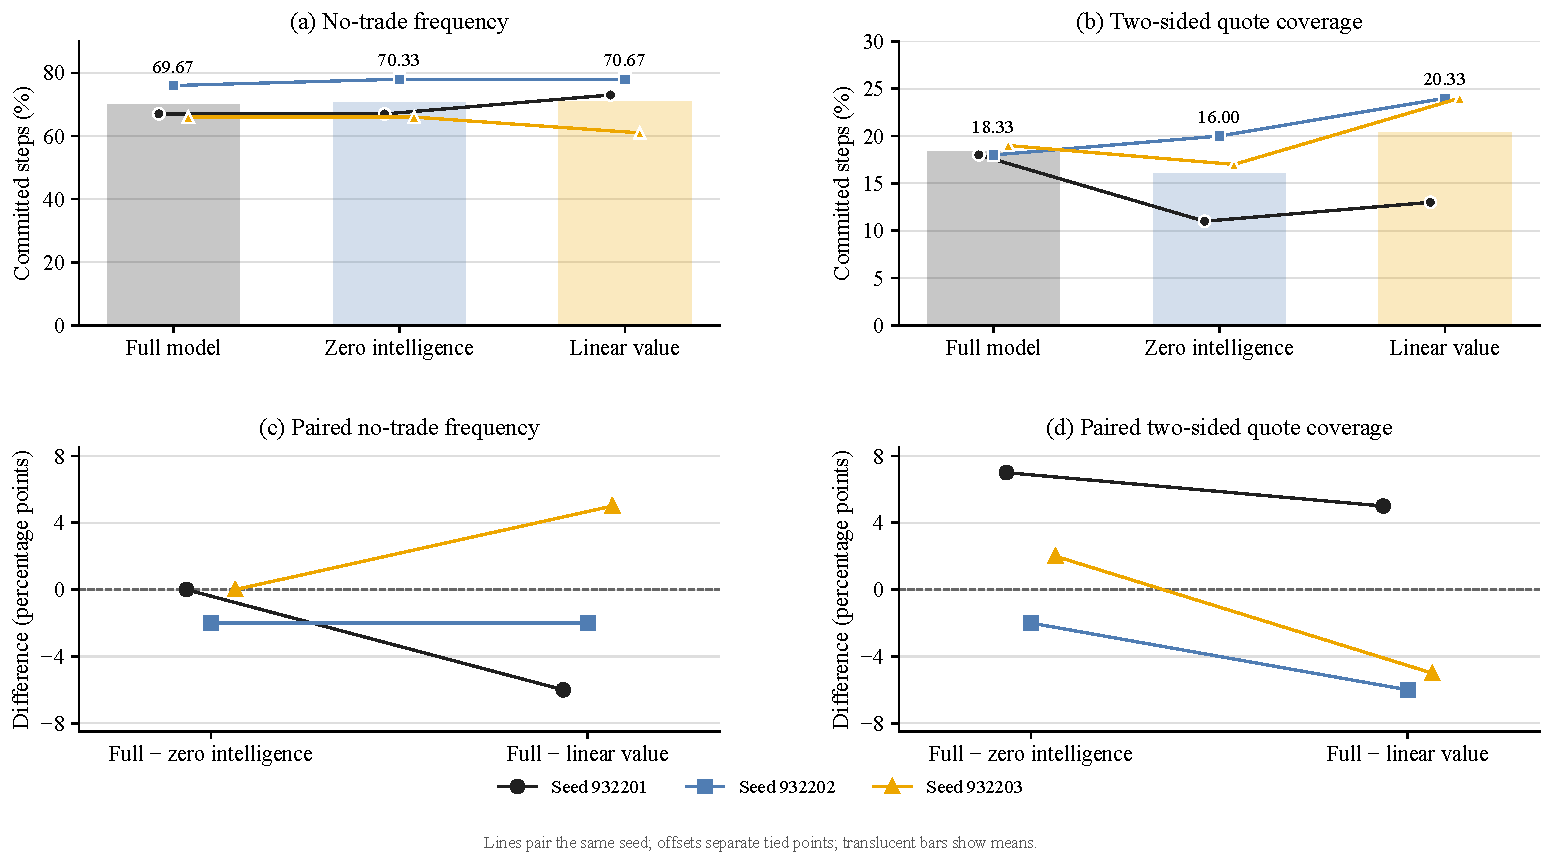
\includegraphics[width=0.96\textwidth]{figures/fig2_rq1_stylized_facts.pdf}
 \caption{九条规则轨迹的日内市场活动。上排为无成交步与双边盘口覆盖率，下排为同一种子下完整模型减去各基线的差值，单位为百分点。上排柱为跨种子均值，点线连接同一种子下的各策略结果。同位置的点略作横移以便辨认。}
 \Description{九条轨迹的市场活动、双边盘口覆盖率与种子内配对差。}
 \label{fig:rq1_zh}
\end{figure*}

\paragraph{盘口覆盖率随配对种子变化。}
在活跃率 0.05、挂单单步有效的配置下，61\%--78\% 的步无成交，11\%--24\% 的步同时存在买卖报价。完整模型平均有 69.67\% 的步无成交，双边报价覆盖率为 18.33\%。零智能基线相应为 70.33\% 和 16.00\%，线性价值基线为 70.67\% 和 20.33\%。完整模型的覆盖率相对零智能基线的种子内差值为 $+7,-2,+2$ 个百分点，相对线性价值基线为 $+5,-6,-5$ 个百分点，覆盖率排序随种子变化（图~\ref{fig:rq1_zh}、表~\ref{tab:rq1_results}）。

报价价差 $10^4(P^{\rm ask}-P^{\rm bid})/P^{\rm mid}$ 的样本为买卖队列同时存在的可交易步。联合报告覆盖率可以明确条件价差的统计分母。每条实测轨迹覆盖一个模型交易日。多日评价方案基于日对数收益率 $r_d=\log(P_d/P_{d-1})$，考察超额峰度、收益率与绝对收益率的自相关，以及成交量与 $|r_d|$ 的相关性~\cite{cont2001empirical}（附录~\ref{app:benchmark_details_zh}）。

\subsection{跨尺度反馈与政策反事实（RQ2）}
\label{sec:exp:rq2_zh}

\begin{figure*}[t]
 \centering
 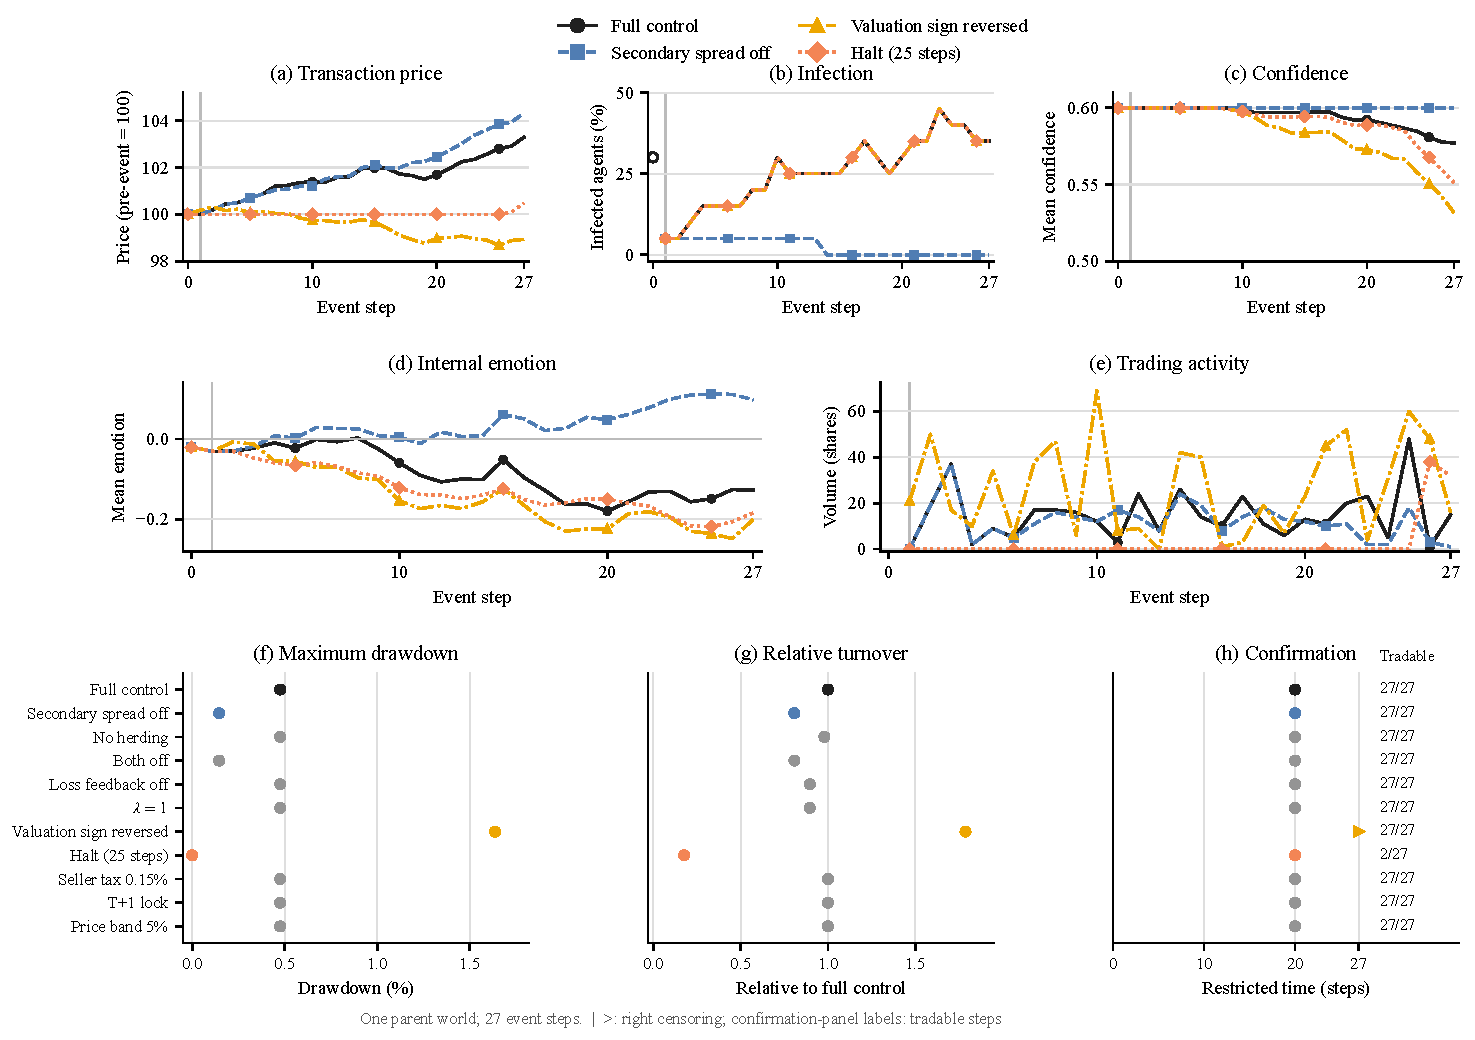
\includegraphics[width=\textwidth]{figures/fig3_rq2_mechanisms_policy.pdf}
 \caption{同一父世界的社会、行为和市场响应。时序面板按同一事件时钟对齐感染比例、模型内部信心与情绪的均值、价格指数及成交股数。图 (b) 的空心点标记事前检查点（20 人中有 6 人感染）。共同事件在 $u=1$ 将全员重置为易感态，再注入一例感染（20 人中有 1 人感染）。下排对照全部十一条分支，箭头标记 $u=27$ 时的右删失。}
 \Description{五组共用事件时间的状态及交易时序，以及三个分支结果面板。}
 \label{fig:rq2_zh}
\end{figure*}

\paragraph{共同检查点分支。}
各分支从种子 933001 的第 5 次提交开始，包含 20 名投资者，每个交易日 4 步，事件窗内每步所有主体均活跃。共同检查点 $u=0$ 已有 6 人处于感染态。在 $u=1$（仿真步 6），共同事件先将全员重置为易感态，再感染一名投资者。因此，事前的 30\% 与首个事件提交步的 5\% 分别对应这次共同重置前后的状态。各分支共用随机流并演化 27 个事件步。图~\ref{fig:rq2_zh}对齐每次提交的感染比例、平均信心与情绪、最新成交价及成交股数。

最大回撤为价格从运行峰值的最大相对跌幅，峰值由事前价格初始化。相对换手率为各分支成交股数除以完整对照的成交股数。价格确认记录首次全局谷底后连续 20 步价格达到事前价格 98\% 时的事件步，谷底可位于 $u=0$。窗口结束时未确认的分支按右删失记录（表~\ref{tab:rq2_results}）。

\paragraph{社会状态与市场响应。}
完整对照的感染率在 $u=23$ 达到 45\%（图~\ref{fig:rq2_zh}b）。平均信心从 $u=10$ 开始走低，窗口结束时为 0.577。平均内部情绪在 $u=20$ 降至 $-0.180$（图~\ref{fig:rq2_zh}c--d）。阻断二次传染后，感染限于初始的一名投资者，到 $u=14$ 清零。该分支的平均信心维持在约 0.600，平均情绪在 $u=25$ 达到 $+0.112$。关闭二次传染也使成交量从 395 股降至 319 股（图~\ref{fig:rq2_zh}e），末步价格指数从 103.28 升至 104.31（图~\ref{fig:rq2_zh}a）。最大回撤从 0.4754\% 降至 0.1453\%，下降 0.3301 个百分点，相对降幅为 69.4\%。

关闭信心依赖从众后，感染峰值仍为 45\%。两条价格路径直到 $u=22$ 都相同，包括决定最大回撤的 $u=15$ 局部峰值和 $u=19$ 谷值，因此两条分支的最大回撤同为 0.4754\%。谷值当步的成交量已相差 1 股，事件窗总成交量从 395 股降至 387 股，相对换手率为 0.9797。令 $Y$ 为最大回撤，两项二元下标分别表示是否启用传染和从众。该父世界中四分支交互项 $Y_{11}-Y_{10}-Y_{01}+Y_{00}$ 为零。

\paragraph{回顾性估值的方向改变价格响应。}
共同事件改变社会状态，价格随其后的实际委托和成交更新。在式~\eqref{eq:aggregate_v_zh}中，价格高于回顾性参考点时，该项对估值的贡献为正。在其他输入固定时，它提高买入倾向，实际委托还取决于其他参考点、情绪及风险容忍度。反转回顾性偏差的符号后，末价较事前低 1.07\%，最大回撤升至 1.6372\%，相对换手率为 1.7873。设 $\lambda=1$ 的分支与进一步移除动态损失反馈的分支均录得 0.4759\% 的回撤及 0.8962 的相对换手率。

\paragraph{交易制度作用于委托与结算的不同环节。}
停牌 25 步后，27 步事件窗内有 2 步可交易，相对换手率为 0.1772，回撤为零。停牌开始时撤去挂单，随后 25 步无成交并沿用上一笔成交价。同期感染率峰值达 45\%，平均内部情绪在 $u=25$ 降至 $-0.218$。$u=26$ 恢复撮合后成交 38 股（图~\ref{fig:rq2_zh}a--e）。其余三个监管分支均保留 27 个可交易步，与对照的 87 笔成交完全相同。5\% 价带分支的委托价与成交价相对各交易日锚价最大偏离为 1.092\%。$T+1$ 锁定股份峰值为 72 股，归档的卖单与成交均未改变。0.15\% 卖方税直接影响结算扣款，在给定状态下式~\eqref{eq:order_quantity_zh}的股数计算保持不变。本事件窗成交相同，卖方税费收入由 20.286250 元增至 60.858750 元。

\paragraph{价格确认的下限反映了短窗口径。}
十个分支的首次谷底位于事前，均在最早可能的第 20 步达到确认条件。停牌分支在持续沿用上一笔成交价时达到该条件。反转估值分支第 25 步触底，之后只有两步，因而在第 27 步右删失。本次比较中所有价格均高于事前的 98\%。此处价格确认反映谷底后的观测步数，需要结合可交易步及换手率解释。

\subsection{决策接口与计算开销（RQ3）}
\label{sec:exp:rq3_zh}

\begin{figure*}[t]
 \centering
 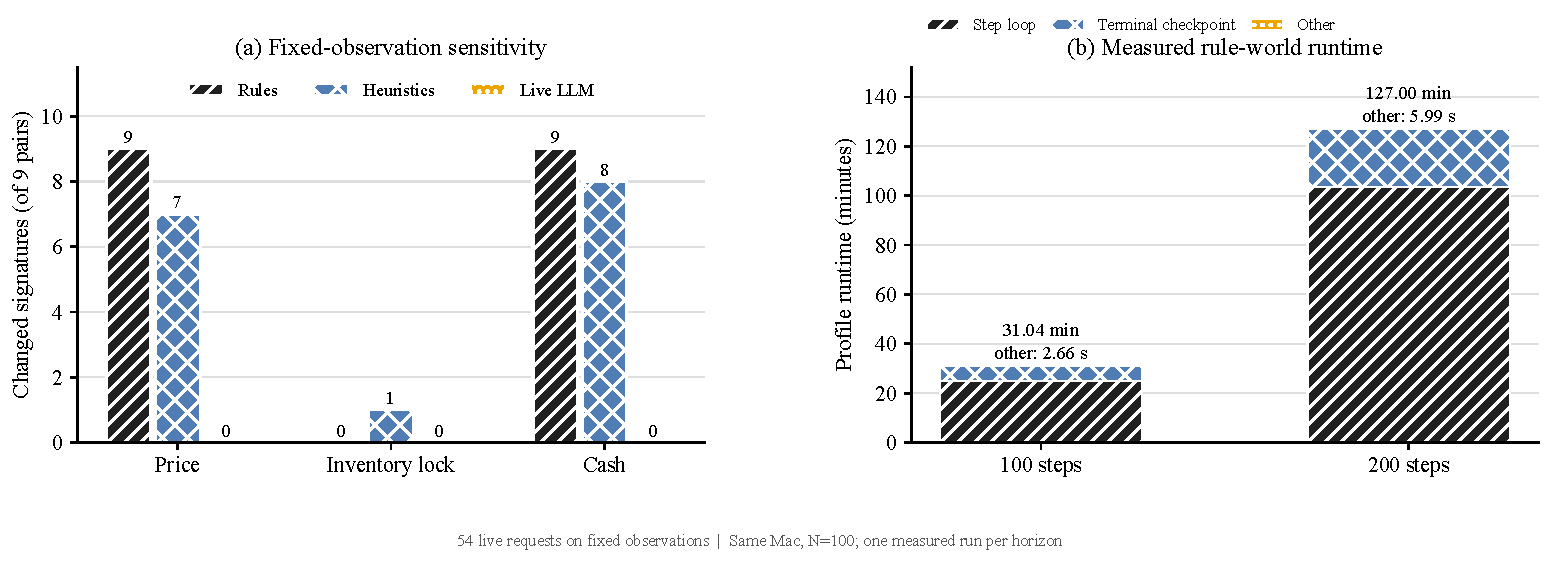
\includegraphics[width=\textwidth]{figures/fig4_rq3_cognition_cost.pdf}
 \caption{固定观察响应与规则世界运行剖面。响应面板给出每类九对观察中的经济动作签名变化数。运行面板拆分同一平台上两次 $N=100$ 规则运行的持久化步循环、终态检查点及其余时间。}
 \Description{三种状态对比的动作签名变化次数与两种仿真期限的分阶段耗时。}
 \label{fig:rq3_zh}
\end{figure*}

\paragraph{固定观察基准检验决策契约。}
九类画像各有价格、锁定股份与现金三种对比，每种对比包含两个状态。中性措辞下共形成 54 个请求单元、45 个不同的构造观察和 27 对比较。采样温度设为零，输出上限为 2,048 tokens。请求配置与归档的 OpenAI API 响应均以 \texttt{gpt-6-luna} 为模型别名。

经济动作签名由方向、带符号股数和限价组成。数值规则在 18/27 对、画像启发式在 16/27 对、LLM 在 0/27 对中改变签名（图~\ref{fig:rq3_zh}a、表~\ref{tab:pilot}）。数值规则输出 45 次买入、9 次观望。发给 LLM 的构造观察同时包含当期状态，以及私有 \texttt{behavior} 字段中保留的模板行为轨迹。54 份请求中，这两份记录的风险和参考价均存在差异。54 份响应均为 \texttt{HOLD}，并通过模式、协议身份、证据 ID 与资源可行性检查。证据检查验证引用 ID 互不重复且属于当次观察的可见集合。签名对比刻画了各后端在这组输入下的响应。要识别字段差异本身的作用，需加入状态与轨迹对齐的对照。

\paragraph{不同画像的委托变化。}
数值规则的价格对比在九类画像中均使带符号股数变化 $-2$ 股，现金对比均变化 $-12$ 股（图~\ref{fig:persona_deltas_zh}）。画像启发式在价格对比中使套利者和平准资金的带符号股数分别变化 $-102$ 股与 $-63$ 股。锁仓对比中，保险机构由卖出 10 股改为 \texttt{HOLD}。在另一组价格对比中，该画像的带符号股数保持不变，限价上移 1,002 个报价档位，对应图中的 $\dagger$。

\begin{figure*}[t]
 \centering
 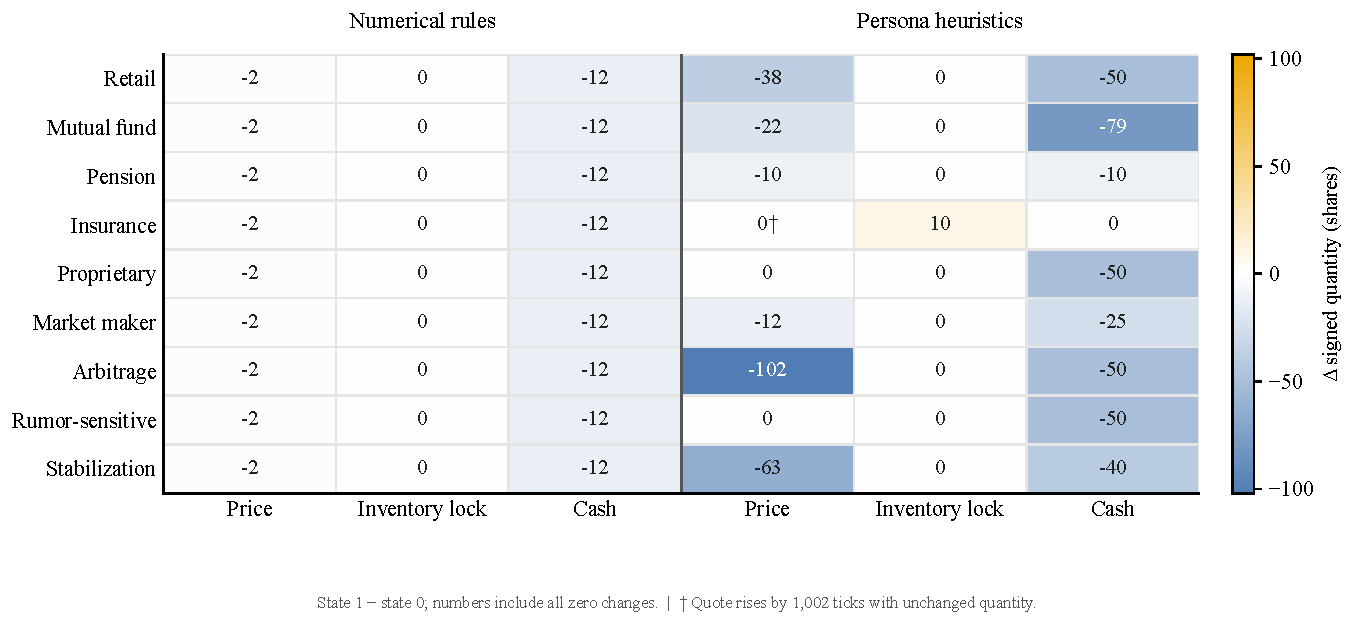
\includegraphics[width=0.96\textwidth]{figures/archetype_order_response.pdf}
 \caption{九类画像的带符号委托量变化。各单元为相应后端和对比下扰动状态减去基准状态的委托股数。买入记正，卖出记负，观望记零。符号 $\dagger$ 标记股数不变而限价变化的单元。}
 \Description{九类画像在数值规则和画像启发式各三种扰动下的带符号委托量变化。}
 \label{fig:persona_deltas_zh}
\end{figure*}

\paragraph{推理开销与公告的计划曝光机会。}
真实请求批次在 69.597 秒内消耗 119,637 个输入 tokens 和 9,306 个输出 tokens，单请求延迟中位数为 2.297 秒。按归档用量和冻结费率核算，成本上界为 0.03456225 美元（表~\ref{tab:rq3_results}）。独立的离线核对在公告发布步求取激活掩码与请求计划的交集。20 个固定种子的公告均落在周期请求步。全量调度共安排 101 次符合资格的请求，周期慢组在 10 个种子中各安排一次。其余 10 个种子在公告发布时均无活跃的慢组主体（图~\ref{fig:schedule_exposure_zh}右图）。式~\eqref{eq:cost_ratio_zh}给出全程的期望请求比例，发布步的计数则显示同一调度如何影响模型接收这次公告的机会。

\paragraph{累计历史的归档处理带来随期限增长的开销。}
在 Apple M5（24 GiB）上，相同种子、100 主体的规则世界由 100 步延长至 200 步时，剖面总耗时由 1,862.397 秒增至 7,619.767 秒，为原来的 4.091 倍。进程内存峰值由 1.239 GiB 增至 2.486 GiB。终态检查点包含已持久化增量链的重建，分别耗时 364.780 秒与 1,394.507 秒。执行、提交、持久化发布与终态检查点合计占两次总耗时的 89.9\% 和 91.0\%，决策阶段分别耗时 2.895 秒和 5.789 秒。

当前归档实现反复验证、复制并哈希累积的决策、回执和账本记录。固定种群且历史规模随 $t$ 线性增长时，每步一次全历史扫描产生 $\sum_{t=1}^{T}\mathcal{O}(t)=\mathcal{O}(T^2)$ 的累计访问成本。该项描述累积历史处理，图~\ref{fig:rq3_zh}记录完整运行器的两次实测。AMD Ryzen AI 7 H 350 平台的千主体规则运行保存了全部 12 步，采样内存峰值为 1.692 GiB，控制器在最终剖面阶段终止。同一个 100 主体、12 步世界的三组配对计时中，标量化严格校验使总用时下降 1.52\%--3.08\%（图~\ref{fig:timing_supp_zh}）。

\section{讨论}
\label{sec:discussion_zh}

\subsection{社会状态如何作用于市场}

市场反馈始于持仓和信息曝光的差异。相近的风险敞口提高既有同伴关系的相对权重。消息送达后，其影响取决于局部感染状态，以及主体信心如何调节个人判断与同伴信号的权重。由此形成的委托在订单簿中与其他委托相遇。结算改变下一步可见的持仓和价格参考点。共同父世界分支将干预前的市场历史固定下来，使这条作用路径可以逐步观测。

在该组比较中，传播和从众改变了不同的市场结果。关闭二次感染后，两条价格路径仍整体上行，但回撤幅度下降。关闭从众后，决定同一最大回撤的谷值价格相同，成交量却已出现差异。结合成交与价格记录，就能在价格路径分化前识别交易活动的变化。反转回顾性估值的符号使价格末值低于起点。结合感染、信心和成交记录，可以区分各机制开关产生的响应；这些效应以给定父世界状态和事件为条件。

\subsection{交易制度决定市场参与条件}

RQ1 的双边盘口覆盖率界定了观察价差所需的交易条件。RQ2 的停牌分支把同样的问题带到成交价上。零回撤和第 20 步的价格确认都来自停牌期间沿用的成交价，同一期间，感染与情绪仍在演化。因此，依据价格判断市场是否消化了冲击，需要结合当时的交易机会与社会状态。其余分支展示三个不同的制度环节。价带限定可接受的报价，交收锁仓改变可卖股数，卖方税在结算时重新分配现金。本次记录中，报价处于价带之内，股份锁定未改变实际卖单，税费在成交相同的条件下改变账本余额。因此，比较制度效果时可以结合委托准入、资金和股份预留、现金结算、价格及换手率。

\subsection{LLM 决策取决于观察时序}

系统将语言模型决策接入规则智能体所用的同一个市场。LLM 可以依据可见消息和账户事实生成委托；类型化意图和整数资源检查使委托遵守统一撮合规则。公开发布使公告进入市场视图。要把公告发送给模型，还需要主体处于活跃状态且当前步符合请求计划。离线核对显示，即使公告落在周期请求步，一半种子的慢组依然没有主体同时满足这两个条件。资源自适应缓存可在请求之后复用交易方向与预算比例。评估这一策略需要同时记录发给模型的观察，以及后来由缓存重新计算的委托。

\subsection{证据范围}

实测路径覆盖一个单资产市场、三个匹配的日内种子，以及一个父世界的干预分支。多日收益分布需要在更长轨迹上使用留出的市场数据验证，独立父世界可用于估计分支效应的变异。双速策略的行为保真度与实际计算开销，需要在状态及轨迹字段一致的闭环中比较。本次固定观察与离线调度基准分别给出接口响应和各类调度提供的观察机会。

\section{结论}
\label{sec:conclusion}

Civitas Economica 将人与人、人与群体和群体与社会的经济关系纳入同一因果时钟。持仓风险改变同伴联系，群体状态进入个体决策，交易所对符合制度约束的委托进行撮合与结算。日内盘口记录显示流动性在何时可观察，共同父世界分支揭示停牌期间平稳价格为何能与恐慌扩散同时出现。决策接口与调度核对进一步追踪哪些信息能够进入不同策略，以及如何比较相应的委托意图。将这些记录与价格和成交对齐，可以回溯价格形成时的交易与信息条件，也可以继续追踪结算后的持仓与估值如何影响下一步。


\label{end:maintext}
\FloatBarrier
\label{start:references}
\bibliographystyle{ACM-Reference-Format}
\bibliography{ref}

\clearpage
\appendix
\section{补充方法细节与提示词架构}
\label{sec:appendix_zh}

\subsection{观察与决策契约}
\label{app:prompt_zh}

观察包含账户、公共市场事实及私人记录。市场视图通过 \texttt{as\_of\_tick} 标记上一步的已提交行情，并提供当步政策状态和事件。私人记录包含画像、更新后的行为状态、所选消息和缓存。认知配置还提供从下一步开始可见的本人近期执行回执。

代码清单~\ref{lst:prompt_zh}示例为符合类型约束的观望响应。主体、观察及版本标识与本次请求对应。后端返回一个观望动作或一张有类型的委托，后者包含资产、方向、股数和整数报价档位。证据标识指向观察内可见事实。交易所在执行阶段校验价格和资源约束。

\noindent\begin{minipage}{\columnwidth}
\begin{lstlisting}[caption={观望动作响应示例。}, label={lst:prompt_zh}, basicstyle=\ttfamily\scriptsize, breaklines=true, frame=single, aboveskip=3pt, belowskip=3pt]
{
  "schema_version": 3,
  "decision_id": "decision-example",
  "actor_id": "agent-example",
  "observation_id": "observation-example",
  "batch_id": "batch-example",
  "observation_version": 1,
  "world_version": 1,
  "tick": 1,
  "policy_id": "kdd27_policy",
  "policy_version": "2",
  "economic_intents": [
    {"kind": "hold", "intent_id": "intent-example"}
  ],
  "evidence_ids": [],
  "belief_patch": {},
  "message_drafts": []
}
\end{lstlisting}
\end{minipage}

\section{基准配置与结果明细}
\label{app:benchmark_details_zh}

\paragraph{多日评价的参考配置。}
表~\ref{tab:params}与表~\ref{tab:behavior}记录长周期参考方案，其中 $N=10{,}000$、$T=20{,}000$、每个交易日 $T_{\rm day}=100$ 步，共 200 个交易日，含 50 日预热。日频协议计算有限样本校正的超额峰度、收益率和绝对收益率的 1--20 阶自相关，以及成交量与绝对收益率的相关性。表~\ref{tab:measured_design}单列本研究实际采用的基准配置。

% Market and Social Layer Default Configurations
\begin{table*}[t]
  \centering\small
  \caption{\tr{长周期参考设计的市场环境与社会传播参数。}{Market and social propagation parameters for the prospective multi-day design.}}
  \label{tab:params}
  \begin{tabularx}{\textwidth}{@{}l p{3.2cm} p{3.5cm} X@{}}
    \toprule
    \tr{模块}{Module} & \tr{参数}{Parameter} & \tr{设置}{Setting} & \tr{含义}{Meaning} \\
    \midrule
    \tr{执行}{Execution} & \tr{主体数、日内步数、仿真期限、预热期}{$N, T_{\mathrm{day}}$, horizon, burn-in} & \tr{$10^4$ 名主体，100 步/日\newline 200 日，预热 50 日}{$10^4$, $100$ steps, $200$ days, $50$ days} & \tr{种群规模、每个交易日的步数、总交易日数与预热日数}{Population, steps per day, horizon, and warm-up} \\
    \tr{账本}{Ledger} & $P_0, \mu_C, \sigma_C, Q_{\max}$ & $100, \log(10^5), 0.6, 2000$ & \tr{初始价格、对数正态现金分布与初始持仓上限}{Initial price, lognormal cash, and maximum initial shares} \\
    \tr{初始禀赋}{Endowments} & $\mu_K, \sigma_K, a_s, b_s$ & $100, 5, 2, 2$ & \tr{截断持仓成本分布与初始情绪 $s_{i,0}\in[-1,1]$ 的对称 Beta 抽样}{Truncated cost and symmetric Beta draws for $s_{i,0} \in [-1, 1]$} \\
    \tr{认知状态}{Cognition} & $q_0, \sigma_{q,0}, a_{i,0}, R^\bullet_{i,0}$ & $0.6, 0.1, 0.5, P_0$ & \tr{信心截断至 $[0,1]$，以及初始风险容忍度与价格参考点}{Confidence truncated to $[0,1]$, risk tolerance, and price anchors} \\
    \tr{网络拓扑}{Topology} & \tr{平均度 $k$、重连概率 $p$}{Mean degree $k$, rewiring $p$} & $6, 0.1$ & \tr{带聚类及短路径的 Watts--Strogatz 网络}{Watts--Strogatz network with clustering and shortcuts} \\
    \tr{边权}{Edge Weights} & $w_0, w_{\min}, w_{\max}, \omega$ & $1.0, 1.0, 2.0, 0.1$ & \tr{边权向 $2-|x_i^{\rm exp}-x_j^{\rm exp}|$ 调整}{Edge weights move toward $2-|x_i^{\rm exp}-x_j^{\rm exp}|$} \\
    \tr{消息筛选}{Information} & \tr{注意力容量 $A_i$、衰减 $\zeta_E$、权重 $\boldsymbol{\theta}$}{Capacity $A_i$, decay $\zeta_E$, weights $\boldsymbol{\theta}$} & $3, 0.05$,\newline$(0.35, 0.25, 0.15, 0.15, 0.10)$ & \tr{按情绪、主题、风险、影响力及曝光记录排序}{Attention-bounded filtering; ranking by emotion, topic, risk, influence, and exposure} \\
    \tr{传播}{Contagion} & \tr{基础感染率 $\beta$、恢复率 $\gamma$、免疫衰减 $\delta$}{Base infection $\beta$, recovery $\gamma$, waning $\delta$} & $0.30, 0.10, 0.05$ & \tr{社会联系上的离散时钟 SIRS 传播参数}{Discrete-time SIRS epidemiological parameters governing panic transmission across social edges} \\
    \tr{感染压力}{Pressure} & \tr{分量权重 $(\kappa_0,\kappa_1,\kappa_2)$}{Coupling weights $(\kappa_0, \kappa_1, \kappa_2)$} & $0.40, 0.40, 0.20$ & \tr{结合感染邻居和注意力筛选后信息的感染压力}{Multiscale infection pressure coupling infected-neighbor share and filtered exposure} \\
    \tr{回音室}{Echo Chamber} & \tr{持续时间 $\eta_d$、回音室 $\eta_e$、再易感 $\eta_\psi$}{Duration $\eta_d$, echo $\eta_e$, resusceptibility $\eta_\psi$} & $0.02, 0.50, 0.50$ & \tr{感染持续时间、曝光集中度与再次易感}{Duration, exposure concentration, and return to susceptibility} \\
    \tr{从众}{Herding} & \tr{悲观阈值 $s_*$、权重转移 $\eta_H$、信心更新 $\eta_q,\eta_{\mathrm{rec}}$}{Threshold $s_*$, shift $\eta_H$, learning $\eta_q, \eta_{\mathrm{rec}}$} & $0.20, 0.50, 0.05, 0.02$ & \tr{信心调节个人估值和同伴信号之间的权重转移}{Panic sentiment boundary; confidence-dependent cognitive weight reallocation to peer consensus} \\
    \tr{市场制度}{Microstructure} & \tr{佣金 $c$、印花税 $\tau^{\mathrm{tax}}$、价带 $L$、价格档位 $\Delta_p$}{Fee $c$, stamp tax $\tau^{\mathrm{tax}}$, band $L$, tick $\Delta_p$} & $0.025\%, 0.05\%, 10\%, 0.01$ & \tr{双边佣金、卖方税、日价格限制与最小报价单位}{Bilateral commission, seller-side transaction tax, daily price fluctuation limit, and price tick} \\
    \tr{订单规则}{Order Rules} & \tr{活跃率 $p_{\mathrm{act}}$、有效期、$T+1$ 限制}{Activity rate $p_{\mathrm{act}}$, lifespan, T+1 limit} & \tr{$p_{\mathrm{act}}=0.05$，有效期 1 步\newline $T+1$ 可配置}{$0.05$, $1$ step, configurable} & \tr{伯努利活跃概率、未成交订单的撤单期限与当日回转限制}{Bernoulli activity probability, unexecuted order cancellation horizon, and day-trade turnover restriction} \\
    \bottomrule
  \end{tabularx}
\end{table*}

% Behavioral and Cognitive Core Parameters
\begin{table*}[t]
  \centering\small
  \caption{\tr{参考设计中的估值、委托与认知参数。}{Valuation, order, and cognition parameters in the reference design.}}
  \label{tab:behavior}
  \begin{tabularx}{\textwidth}{@{}l p{3.2cm} p{3.5cm} X@{}}
    \toprule
    \tr{模块}{Module} & \tr{参数}{Parameter} & \tr{设置}{Setting} & \tr{含义}{Meaning} \\
    \midrule
    \tr{前景理论}{Prospect Theory} & \tr{损失厌恶 $\lambda_i$、幂指数 $\alpha$、缩放系数 $\kappa_v$}{Loss aversion $\lambda_i$, power $\alpha$, scale $\kappa_v$} & \mbox{2.25, 0.88, 10} & \tr{参考依赖价值函数。$\alpha$ 与 $\lambda$ 取自文献，$\kappa_v$ 为模型设定}{Reference-dependent value; $\alpha$ and $\lambda$ follow literature values, $\kappa_v$ is a model choice} \\
    \tr{参考点更新}{Reference Dynamics} & \tr{记忆速率 $(\kappa_p, \kappa_h, \kappa_n, \kappa_e)$}{Memory rates $(\kappa_p, \kappa_h, \kappa_n, \kappa_e)$} & $(0.03, 0.10, 0.16, 0.18)$ & \tr{持仓成本、滚动高点、同伴与政策参考点的更新速率}{Adaptive update rates for purchase cost, local rolling peak, peer consensus, and policy anchor} \\
    \tr{参考点权重}{Reference Weights} & \tr{参考点权重 $(\omega_p, \omega_h, \omega_n, \omega_e)$}{Anchor weights $(\omega_p, \omega_h, \omega_n, \omega_e)$} & $(0.34, 0.26, 0.20, 0.20)$ & \tr{多参考点心理账户，滚动窗口 $H_h=100$ 步，参考点目标幅度 $\xi_n=\xi_e=0.05$}{Multi-reference mental accounting; $H_h = 100$ rolling steps, reference-target amplitudes $\xi_n = \xi_e = 0.05$} \\
    \tr{损失压力}{Loss Pressure} & \tr{敏感度 $\chi$、上下界 $[\ell_{\min},\ell_{\max}]$、损失缩放 $\nu$}{Coupling $\chi$, bounds $[\ell_{\min}, \ell_{\max}]$, loss-penalty scale $\nu$} & \tr{$\chi=0.50$，$[1.0,5.0]$\newline $\nu=4.0$}{$0.50, [1.0, 5.0], 4.0$} & \tr{由持仓成本及近期高点驱动的损失压力}{Reference-loss pressure based on cost and high-price anchors} \\
    \tr{风险容忍度}{Risk Preference} & \tr{动态权重 $\boldsymbol{\omega}_a$}{Dynamic weights $\boldsymbol{\omega}_a$} & $(0.35, 0.45, 0.10, 0.10, 0.15)$ & \tr{信心、上一期风险容忍度、情绪、估值方向、损失惩罚权重}{Weights on confidence, previous risk, emotion, direction, and loss penalty} \\
    \tr{订单生成}{Order Generation} & \tr{缩放系数 $\kappa_a$、阈值 $\delta_a$、投入范围 $[f_{\min},f_{\max}]$}{Scale $\kappa_a$, threshold $\delta_a$, limits $[f_{\min}, f_{\max}]$} & $5.0, 0.25, [0.01, 0.10]$ & \tr{交易意图至委托的映射及资源投入比例}{Intent-to-order mapping; fraction of available liquidity deployed per active trading step} \\
    \tr{交易意图}{Intention} & \tr{权重 $(\omega_\tau^d,\omega_\tau^s,\omega_\tau^a)$}{Weights $(\omega_\tau^d,\omega_\tau^s,\omega_\tau^a)$} & $(0.45,0.40,0.15)$ & \tr{估值方向、情绪与风险容忍度权重}{Valuation direction, sentiment, and risk tolerance} \\
    \tr{报价}{Quote Pricing} & \tr{扰动 $\sigma_p$、价格档位 $\Delta_p$}{Perturbation $\sigma_p$, tick size $\Delta_p$} & $0.002, 0.01$ & \tr{以上一提交价格为中心作均值校正的对数正态扰动}{Mean-corrected log-normal quote dispersion around the previous committed price} \\
    \tr{情绪权重}{Emotion Weights} & \tr{技术型、新闻型、从众型}{Technical / News / Herding styles} & \shortstack[l]{$(.6,.1,.1,.2)$\\$(.35,.35,.2,.1)$\\$(.25,.15,.5,.1)$} & \tr{不同风格的惯性、感染、同伴与上一期收益权重}{Weights on inertia, infection, peers, and prior return by cognitive style} \\
    \tr{双速混合调度}{Dual-Speed Hybrid} & \tr{慢组人数 $k$、周期 $T_{\mathrm{slow}}$、缓存寿命 $A_{\max}$}{Count $k$, period $T_{\mathrm{slow}}$, cache TTL $A_{\max}$} & \tr{$10$、10 步、10 步}{$10, 10\text{ steps}, 10\text{ steps}$} & \tr{认知参考配置的慢组人数、请求周期与缓存有效期}{Slow group size, request period, and cache lifetime in the cognition profile} \\
    \tr{主体记忆}{Agent Memory} & \tr{衰减尺度 $S_m$、最大条目 $M_{\max}$}{Decay factor $S_m$, max items $M_{\max}$} & \tr{$100$ 步、8}{$100\text{ steps}, 8$} & \tr{主体自己的近期执行回执与记忆衰减尺度}{Own execution receipts and their decay scale in the cognition profile} \\
    \bottomrule
  \end{tabularx}
\end{table*}


\paragraph{基准结果明细。}
表~\ref{tab:invariants}逐条报告账本核验。表~\ref{tab:rq1_results}汇总日内轨迹，表~\ref{tab:rq2_results}报告全部共同父世界分支的结果。表~\ref{tab:pilot}和表~\ref{tab:rq3_results}分别记录决策计数与计算开销。

\begin{table*}[t]
  \centering\small
  \caption{\tr{各匹配种子的账本守恒与终态恢复。同平台只读恢复结果与各归档的终态哈希一致。}{Ledger conservation and terminal restoration for each matched seed. Read-only restorations on the same platform reproduce the archived terminal state hashes.}}
  \label{tab:invariants}
  \begin{tabularx}{\textwidth}{@{}l X r r r r c@{}}
    \toprule
    \tr{种子}{Seed} & \tr{交易策略}{Trading policy} & \tr{提交步数}{Commits} & \tr{现金残差}{Cash residual} & \tr{股份残差}{Share residual} & \tr{税费残差}{Fee residual} & \tr{终态哈希}{Terminal hash}\\
    \midrule
    932201 & \tr{完整模型}{Full model} & 100 & 0 & 0 & 0 & \tr{匹配}{Match} \\
    932201 & \tr{零智能}{Zero intelligence} & 100 & 0 & 0 & 0 & \tr{匹配}{Match} \\
    932201 & \tr{同质线性价值}{Linear value} & 100 & 0 & 0 & 0 & \tr{匹配}{Match} \\
    932202 & \tr{完整模型}{Full model} & 100 & 0 & 0 & 0 & \tr{匹配}{Match} \\
    932202 & \tr{零智能}{Zero intelligence} & 100 & 0 & 0 & 0 & \tr{匹配}{Match} \\
    932202 & \tr{同质线性价值}{Linear value} & 100 & 0 & 0 & 0 & \tr{匹配}{Match} \\
    932203 & \tr{完整模型}{Full model} & 100 & 0 & 0 & 0 & \tr{匹配}{Match} \\
    932203 & \tr{零智能}{Zero intelligence} & 100 & 0 & 0 & 0 & \tr{匹配}{Match} \\
    932203 & \tr{同质线性价值}{Linear value} & 100 & 0 & 0 & 0 & \tr{匹配}{Match} \\
    \bottomrule
  \end{tabularx}
\end{table*}

% Generated from packaged archive data by scripts/render_real_figures.py
\begin{table*}[t]
\centering\small
\caption{\tr{RQ1 日内市场活动与盘口流动性。每种模型包含三个匹配种子的轨迹（$N=100,T=100$）。各指标报告均值及 [最小值, 最大值]。}{RQ1 Intraday Market Activity and Quoted Liquidity. Each model has three matched-seed trajectories ($N=100,T=100$). Entries report mean [minimum, maximum].}}
\label{tab:rq1_results}
\begin{tabularx}{\textwidth}{@{}l r X X X X@{}}
\toprule
Baseline & Worlds & No trade (\%) & One-sided book (\%) & Two-sided quotes (\%) & Trades \\
\midrule
Civitas full model & 3 & 69.67 [66, 76] & 71.67 [69, 76] & 18.33 [18, 19] & 43.67 [34, 57] \\
Zero intelligence & 3 & 70.33 [66, 78] & 70.67 [68, 73] & 16.00 [11, 20] & 42.67 [34, 50] \\
Homogeneous linear value & 3 & 70.67 [61, 78] & 68.33 [64, 73] & 20.33 [13, 24] & 44.67 [36, 55] \\
\bottomrule
\end{tabularx}
\end{table*}

% Generated from packaged archive data by scripts/render_real_figures.py
\begin{table*}[t]
\centering\small
\caption{\tr{RQ2 共同父世界的十一条干预分支（$N=20$，27 步事件窗口）。感染峰值取事件窗口内逐步感染比例的最大值。星号标记窗口终点的右删失。}{RQ2 Outcomes for Eleven Intervention Branches from a Shared Parent World ($N=20$, 27 event steps). Peak infection is the maximum stepwise infection share within the event window. An asterisk marks right censoring at the window endpoint.}}
\label{tab:rq2_results}
\begin{tabularx}{\textwidth}{@{}l c c c c c X@{}}
\toprule
Intervention & MDD (\%) & Peak infection (\%) & Relative turnover & Confirmation (steps) & Censored & Tradable steps \\
\midrule
Full control & 0.4754 & 45 & 1.0000 & 20 & No & 27/27 \\
Secondary spread off & 0.1453 & 5 & 0.8076 & 20 & No & 27/27 \\
No herding & 0.4754 & 45 & 0.9797 & 20 & No & 27/27 \\
Both off & 0.1453 & 5 & 0.8076 & 20 & No & 27/27 \\
Loss feedback off & 0.4759 & 45 & 0.8962 & 20 & No & 27/27 \\
$\lambda=1$ & 0.4759 & 45 & 0.8962 & 20 & No & 27/27 \\
Valuation sign reversed & 1.6372 & 45 & 1.7873 & 27$^{*}$ & Yes & 27/27 \\
Halt (25 steps) & 0.0000 & 45 & 0.1772 & 20 & No & 2/27 \\
Seller tax 0.15\% & 0.4754 & 45 & 1.0000 & 20 & No & 27/27 \\
T+1 lock & 0.4754 & 45 & 1.0000 & 20 & No & 27/27 \\
Price band 5\% & 0.4754 & 45 & 1.0000 & 20 & No & 27/27 \\
\bottomrule
\end{tabularx}
\end{table*}

\begin{table*}[t]
  \centering\small
  \caption{\tr{九类画像及三类配对对比的固定观察响应。各后端均在相同的 54 个请求单元上评价。变化计数以每类九对为分母。}{Fixed-observation responses across nine archetypes and three paired contrasts. All backends use the same 54 cells. Signature changes are counted out of nine pairs per contrast.}}
  \label{tab:pilot}
  \begin{tabularx}{\textwidth}{@{}X rrr c ccc@{}}
    \toprule
    \tr{决策后端}{Backend} & HOLD & BUY & SELL & \tr{资源可行}{Resource feasible} &
    \tr{价格签名变化}{Price changes} & \tr{锁定签名变化}{Lock changes} & \tr{现金签名变化}{Cash changes} \\
    \midrule
    \tr{数值规则}{Numerical rules} & 9 & 45 & 0 & 54/54 & 9/9 & 0/9 & 9/9 \\
    \tr{画像启发式}{Persona heuristics} & 27 & 9 & 18 & 54/54 & 7/9 & 1/9 & 8/9 \\
    \tr{真实 LLM}{Live LLM} & 54 & 0 & 0 & 54/54 & 0/9 & 0/9 & \mbox{0/9} \\
    \bottomrule
  \end{tabularx}
\end{table*}

% Generated from packaged archive data by scripts/render_real_figures.py
\begin{table*}[t]
\centering\small
\caption{\tr{模型请求与规则世界的实测计算记录。$^{a}$ 快照批次壁钟时间。规则世界的运行剖面包括终态检查点。$^{b}$ ASUS 内存为采样峰值，最终运行剖面缺失。}{Measured Compute for Model Requests and Rule Worlds. $^{a}$~Snapshot batch wall time. Rule-world profiles include terminal checkpoints. $^{b}$~ASUS memory is the sampled peak. Its final profile is unavailable.}}
\label{tab:rq3_results}
\begin{tabularx}{\textwidth}{@{}l r c c c X@{}}
\toprule
Measured workload & Live calls & Input / output tokens & Time (s) & Memory (GiB) & Completion status \\
\midrule
Live snapshot batch & 54 & 119,637 / 9,306 & 69.597$^{a}$ & --- & 54/54 responses; all HOLD \\
Mac: $N=100,T=100$ & 0 & 0 / 0 & 1862.397 & 1.239 & Runner/controller complete \\
Mac: $N=100,T=200$ & 0 & 0 / 0 & 7619.767 & 2.486 & Runner/controller complete \\
ASUS: $N=1000,T=12$ & 0 & 0 / 0 & Missing & 1.692$^{b}$ & Runner saved 12 steps; controller stopped \\
\bottomrule
\end{tabularx}
\end{table*}


\section{调度与校验器诊断}
\label{app:timing_zh}

调度核对使用 $N=100$、$T=4{,}000$ 的认知参考配置及 20 个固定种子的活跃掩码。在仿真步 1,200，所有主体的市场视图均含有公告。按计划发出包含文本的请求，需要主体在该步活跃并符合模型请求资格。图~\ref{fig:schedule_exposure_zh}右图给出逐种子计数。

两种严格校验器处理同一个 $N=100$、$T=12$ 的规则世界。图~\ref{fig:timing_supp_zh}给出三组配对计时。

\begin{figure*}[t]
 \centering
 \begin{subfigure}{0.96\textwidth}
  \centering
  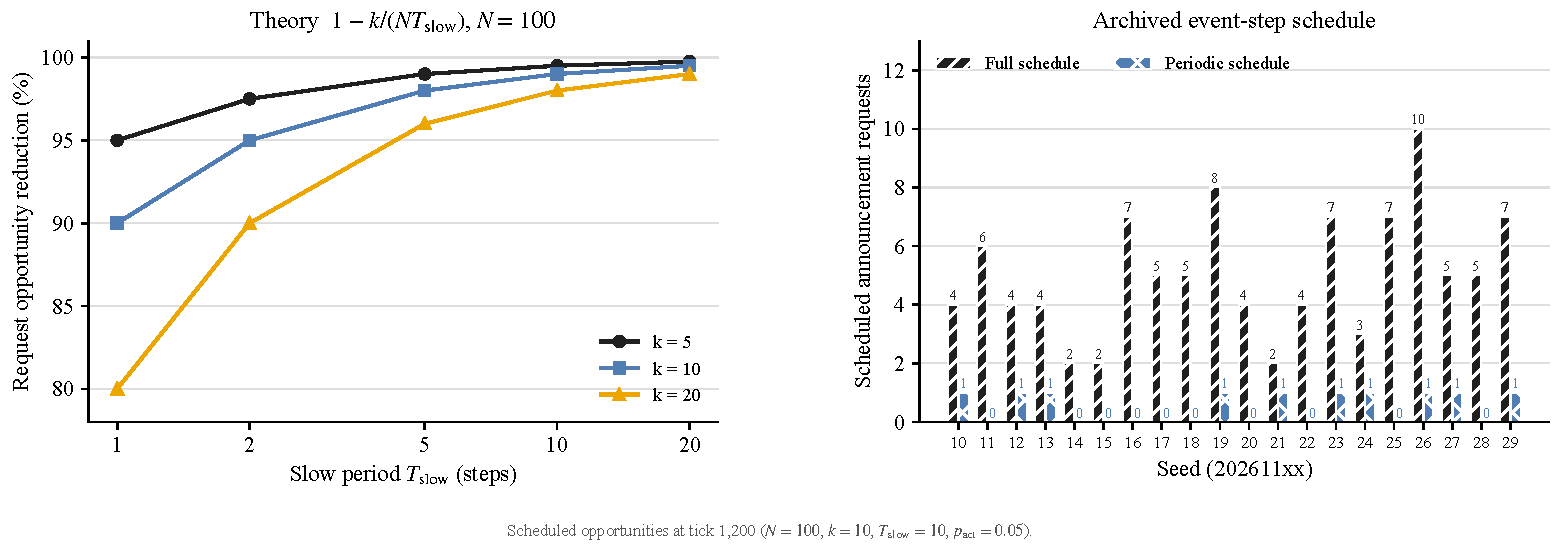
\includegraphics[width=\textwidth]{figures/schedule_exposure.pdf}
  \caption{期望请求缩减与公告请求资格。}
  \label{fig:schedule_exposure_zh}
 \end{subfigure}
 \par\medskip
 \begin{subfigure}{0.55\textwidth}
  \centering
  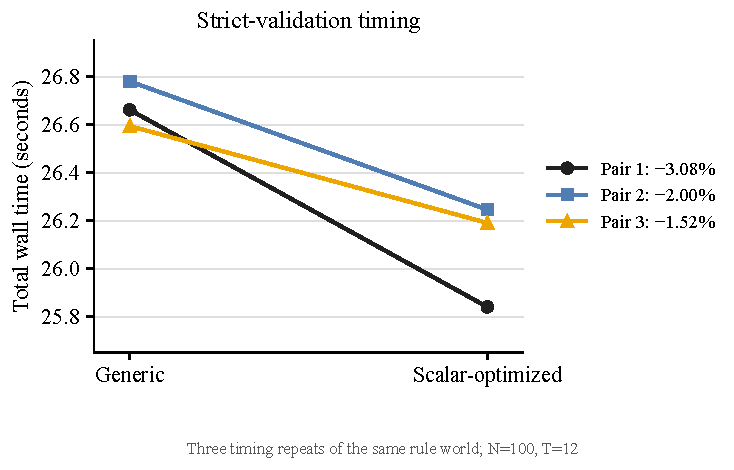
\includegraphics[width=\textwidth]{figures/engineering_timing.pdf}
  \caption{两种严格校验器的配对壁钟耗时。}
  \label{fig:timing_supp_zh}
 \end{subfigure}
 \caption{调度与校验器诊断。（a）左图设 $N=100$、期限为周期整数倍，改变周期 $T_{\mathrm{slow}}$ 与慢组人数 $k$。右图记录公告发布时具备请求资格的活跃主体数。（b）各条连线连接同一规则世界下通用与标量优化校验器的配对计时。}
 \Description{调度的期望请求缩减率、20 个种子的公告请求资格计数和严格校验配对计时。}
\end{figure*}


\end{document}
